\subsection{Descriptive Statistics}
Salary is right-skewed with substantial variability across roles and seniority levels. Descriptive summaries indicate clear gradients by company location and work arrangement. Distributions are visualized in Figure~\ref{fig:salary-dist} and Figure~\ref{fig:salary-box}.

\begin{figure}[H]
  \centering
  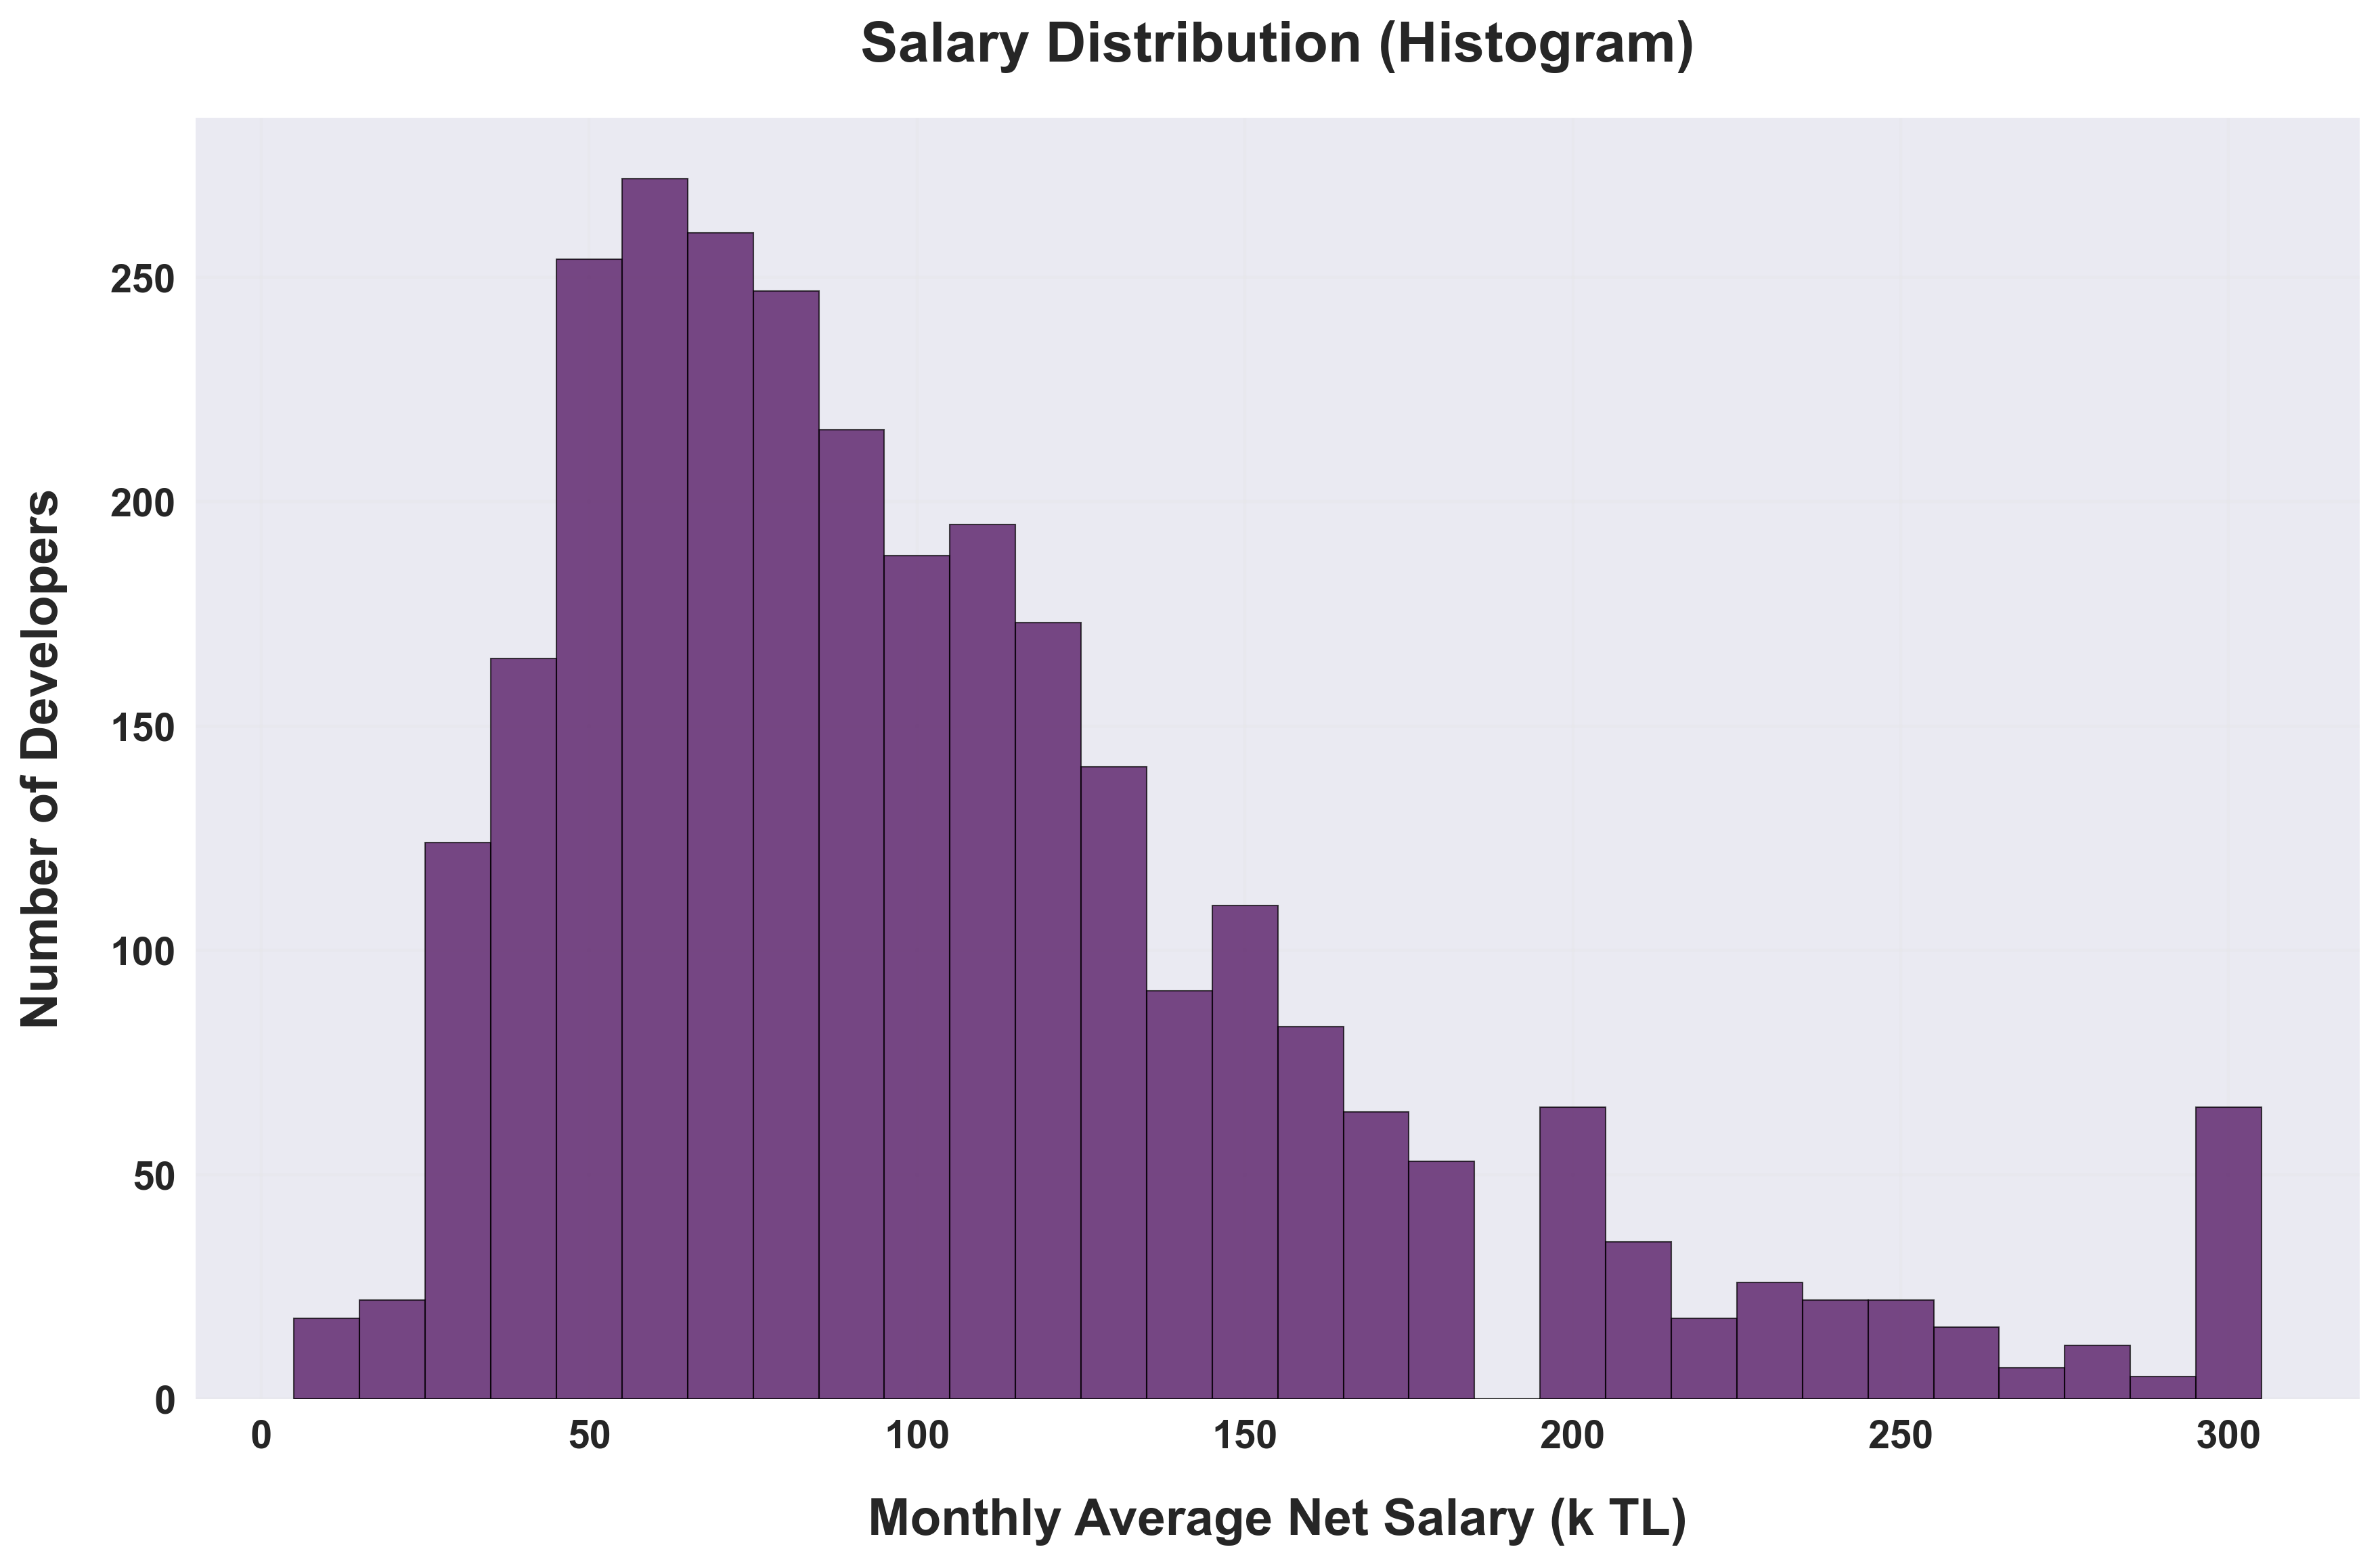
\includegraphics[width=0.85\linewidth]{figures/01_maas_dagilimi_histogram.png}
  \caption{Salary distribution (histogram with density overlay).}
  \label{fig:salary-dist}
\end{figure}

\begin{figure}[H]
  \centering
  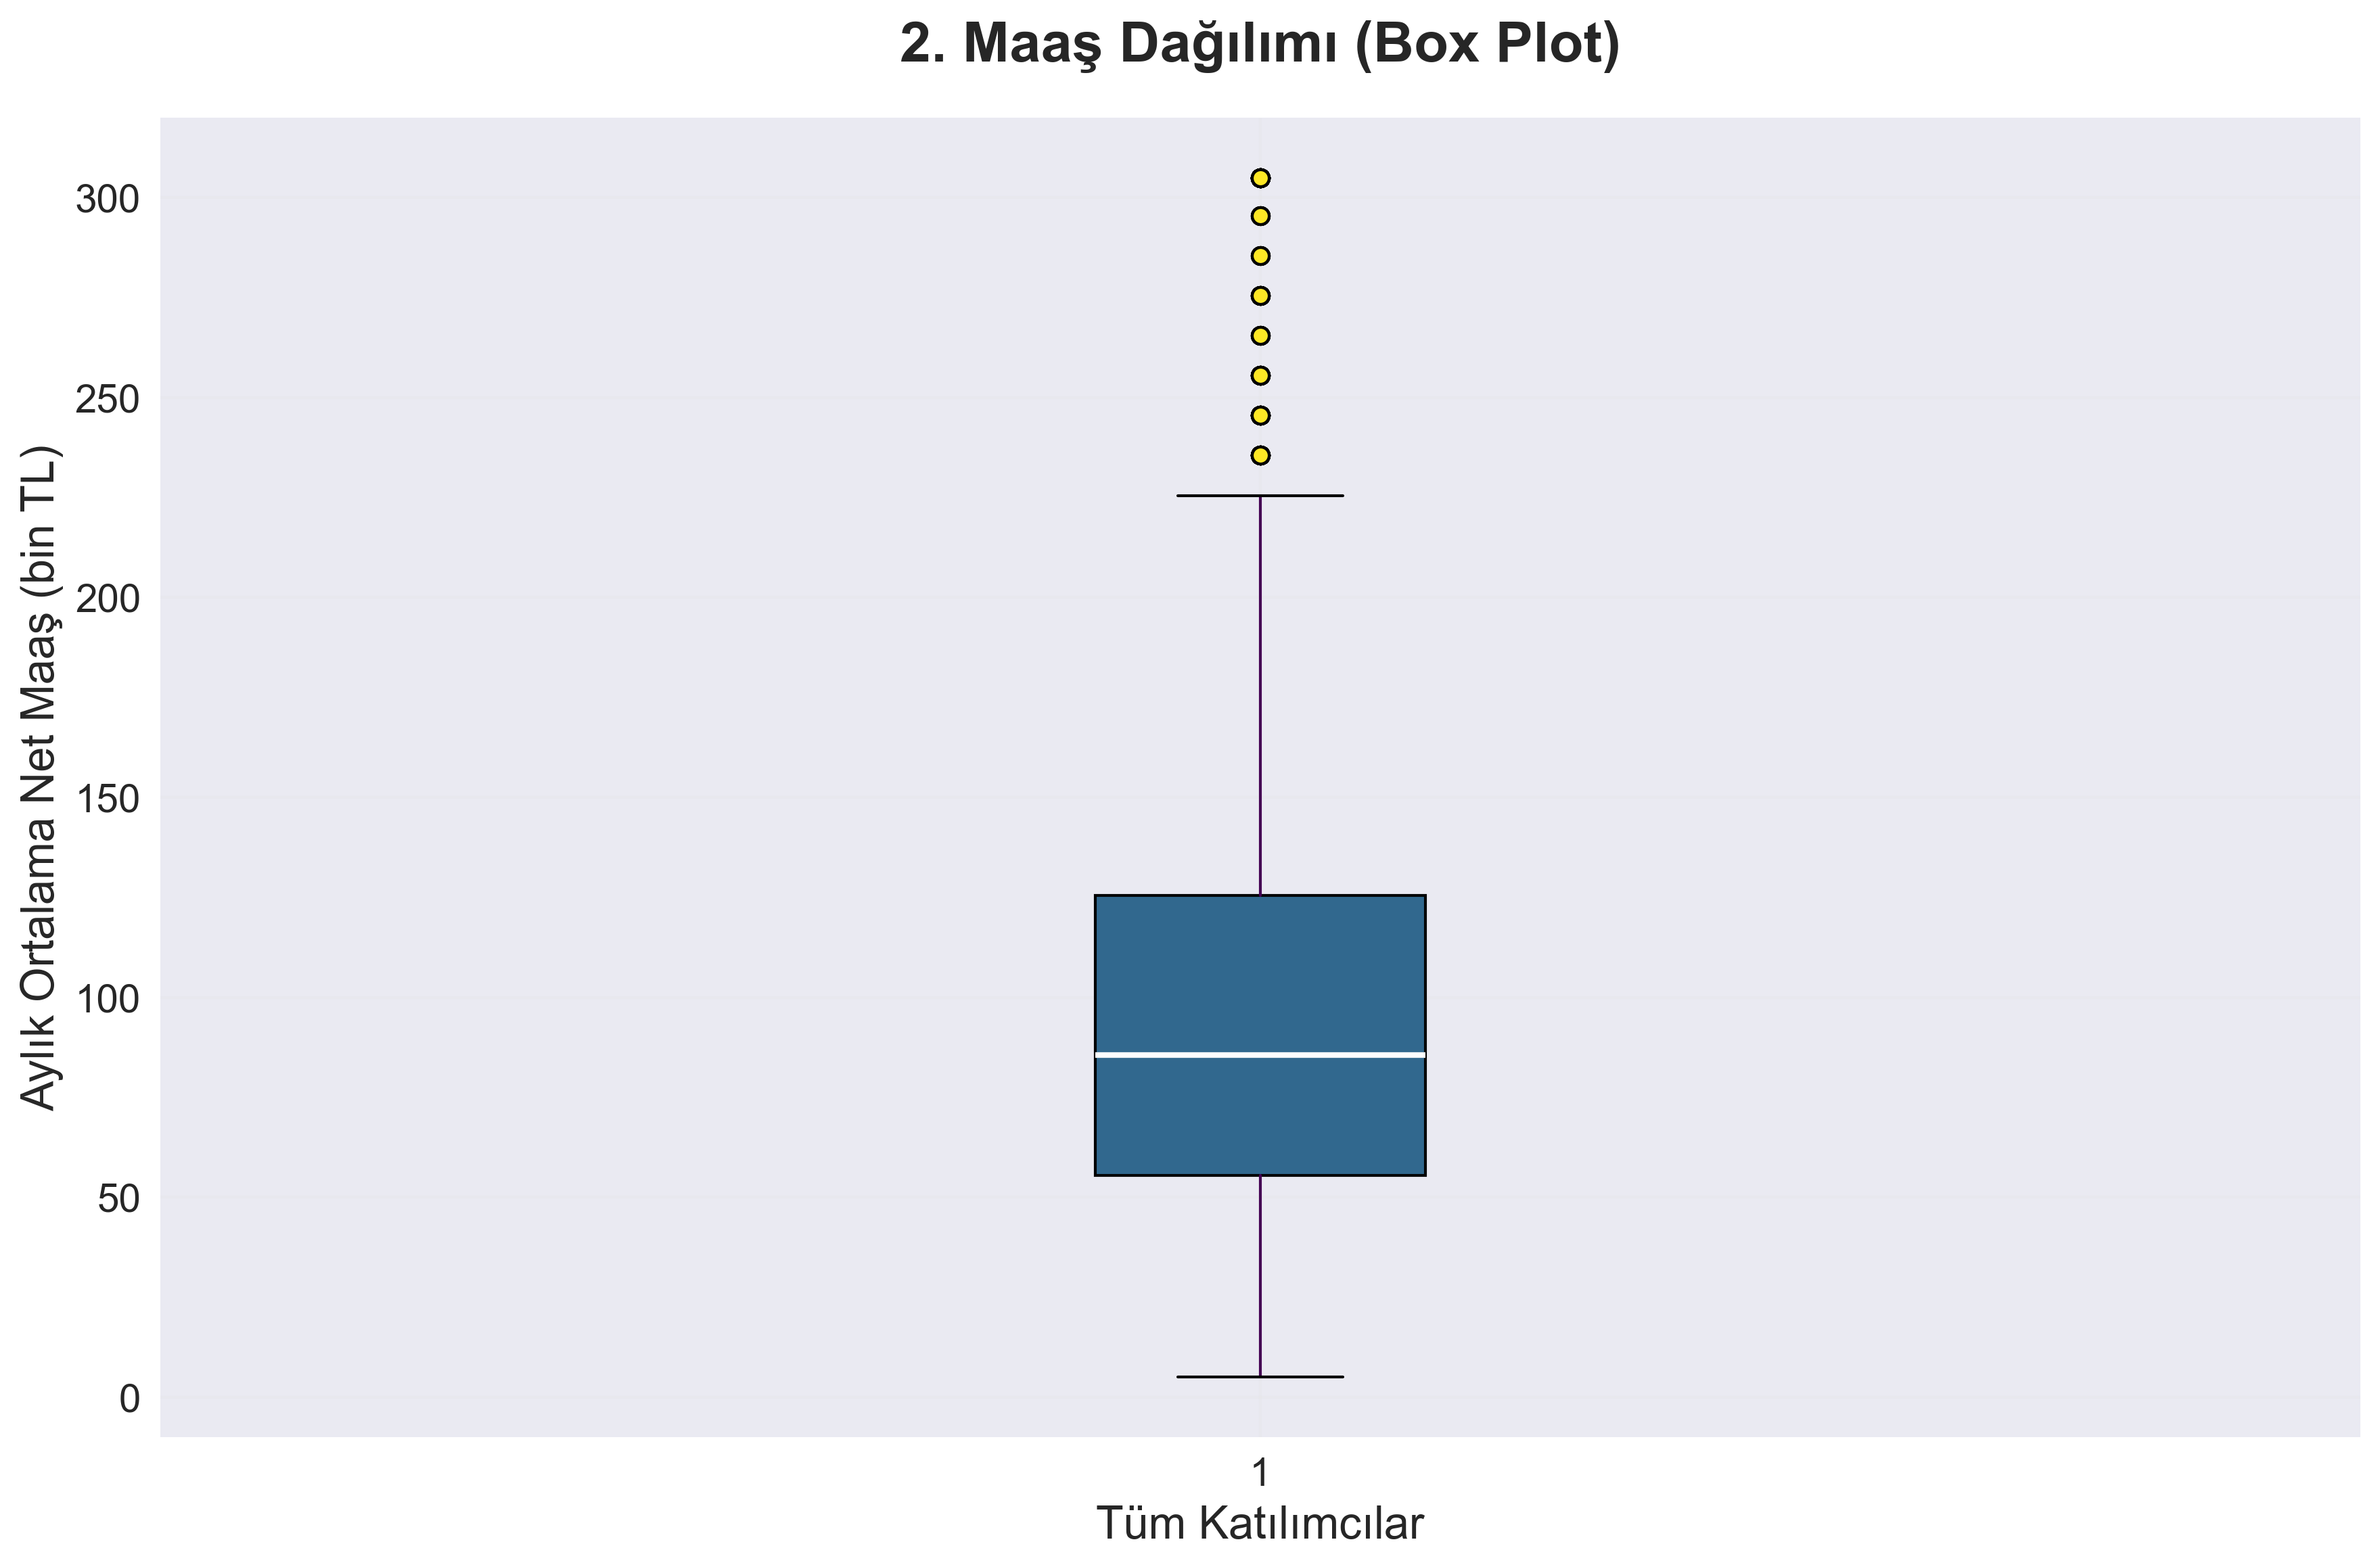
\includegraphics[width=0.85\linewidth]{figures/02_maas_dagilimi_boxplot.png}
  \caption{Salary distribution (box plot).}
  \label{fig:salary-box}
\end{figure}

\subsection{Hypothesis Testing}
Primary hypothesis tests yielded the following results:
\begin{itemize}[leftmargin=*]
  \item React vs Non-React (independent \textit{t}-test): not statistically significant ($p = 0.228$).
  \item Work arrangement (one-way ANOVA): statistically significant ($p < 0.001$), medium effect size.
  \item Company location (one-way ANOVA): statistically significant ($p < 0.001$), large effect size.
  \item Gender pay gap (independent \textit{t}-test): statistically significant ($p = 0.0004$), mean gap $\approx 16\%$.
\end{itemize}

Post-hoc comparisons (Tukey HSD) indicate differences are concentrated between remote vs office and by clusters of company locations.

\subsection{Stack ROI}
We benchmarked mean salaries by programming languages, frontend frameworks, and tools, and summarized relative effect sizes as a qualitative ROI ranking. Stacks combining modern frontend and robust backend competencies tend to outperform single-technology profiles. Figure~\ref{fig:stack-roi} shows the ranked comparison.

\begin{figure}[H]
  \centering
  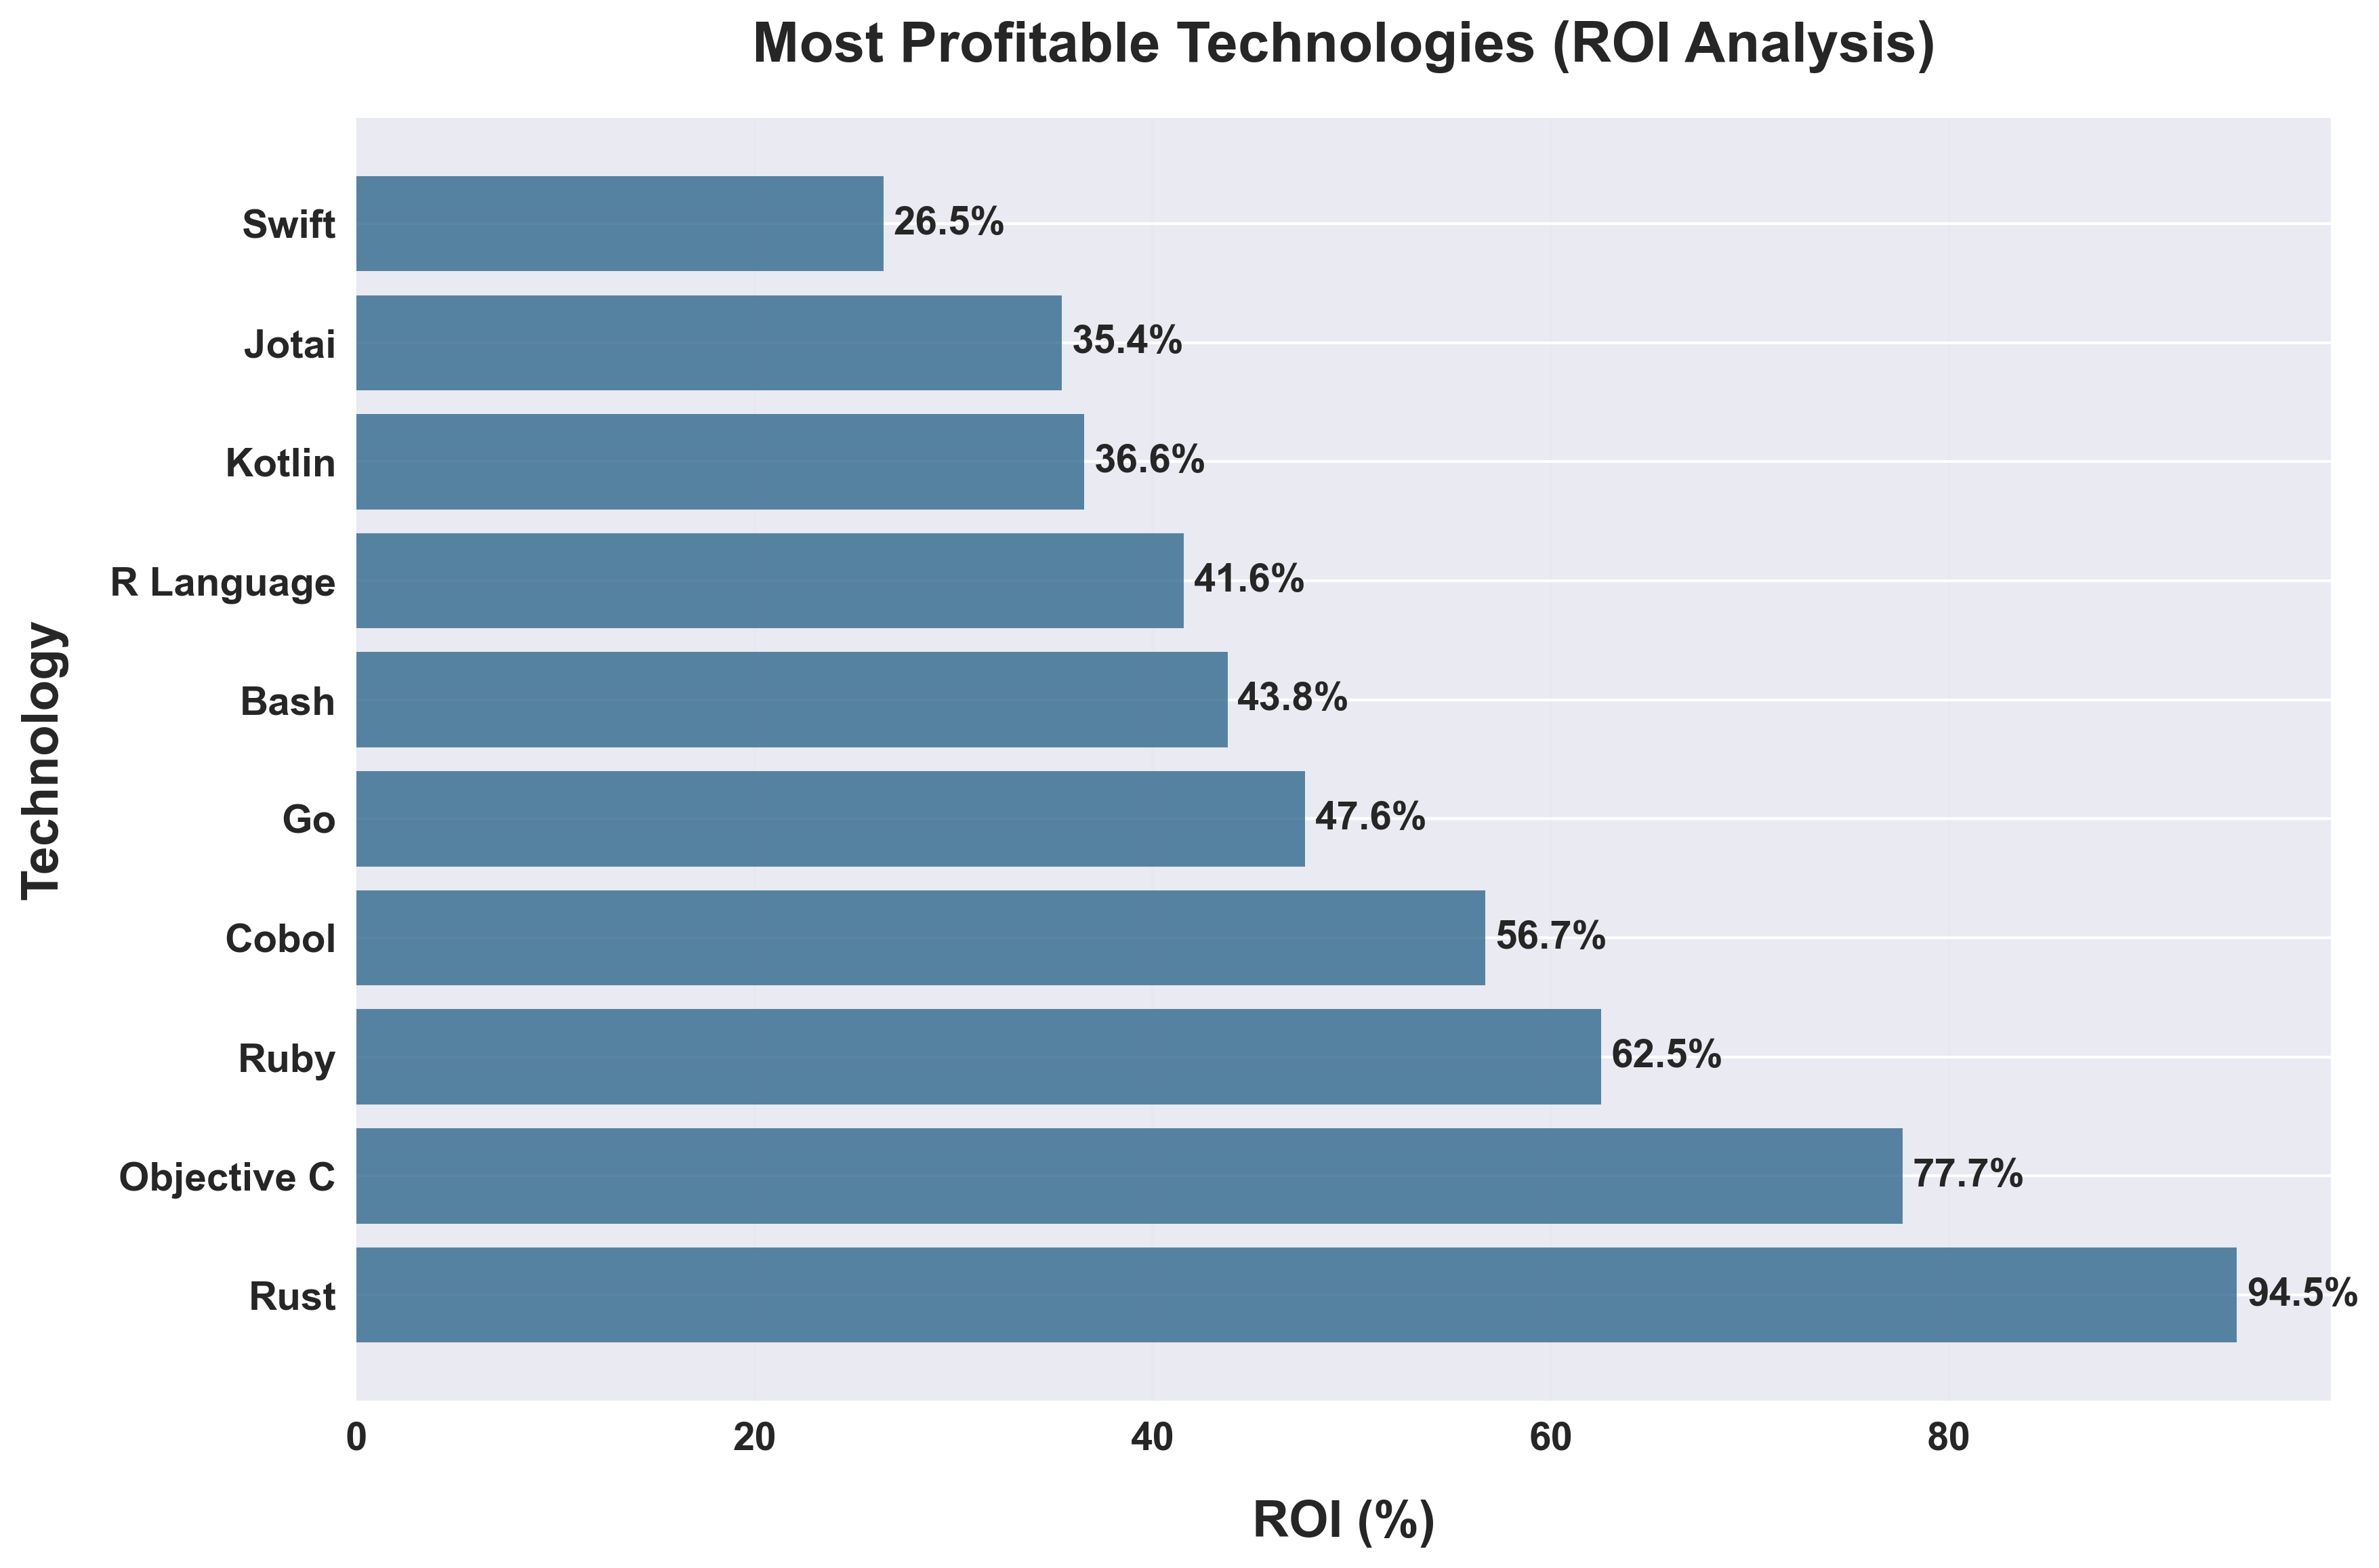
\includegraphics[width=0.85\linewidth]{figures/12_en_karli_teknolojiler.png}
  \caption{Relative ROI by technology stack.}
  \label{fig:stack-roi}
\end{figure}

\subsection{Additional Visualizations}
We include a non-exhaustive set of publication-quality charts to illustrate key relationships:

\begin{figure}[H]
  \centering
  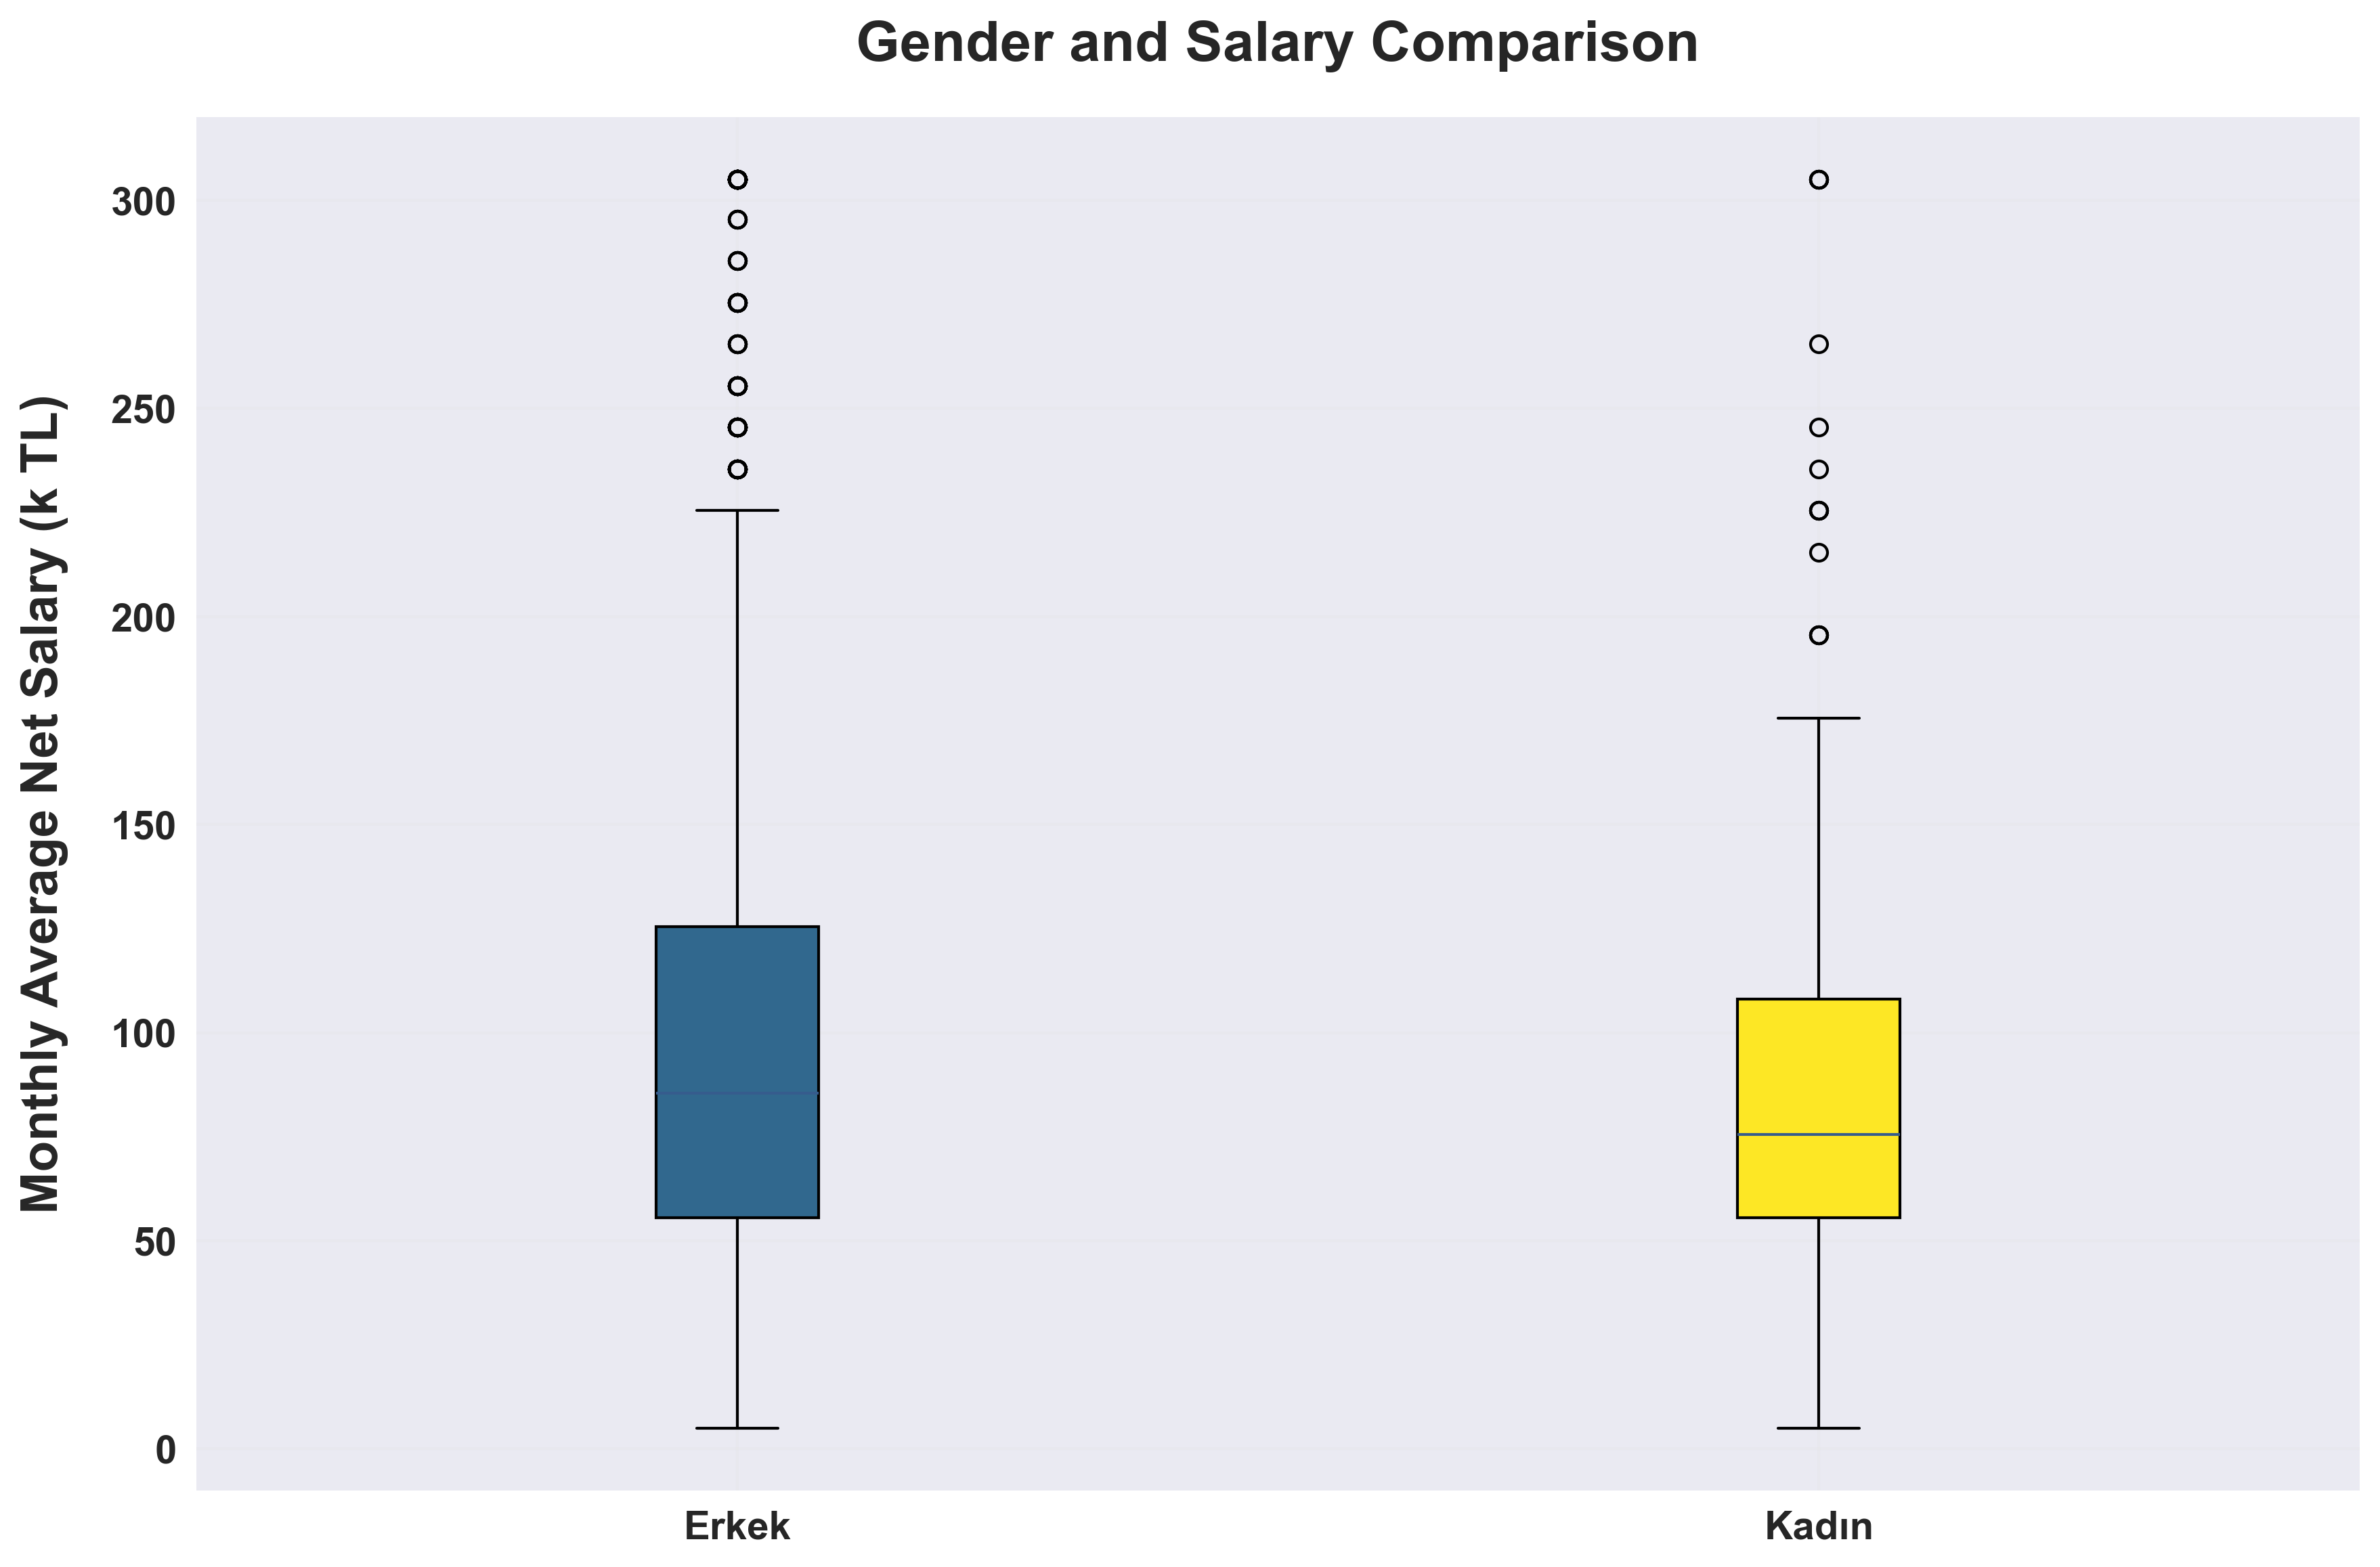
\includegraphics[width=0.85\linewidth]{figures/06_cinsiyet_maas_karsilastirma.png}
  \caption{Gender-based salary comparison.}
  \label{fig:gender-gap}
\end{figure}

\begin{figure}[H]
  \centering
  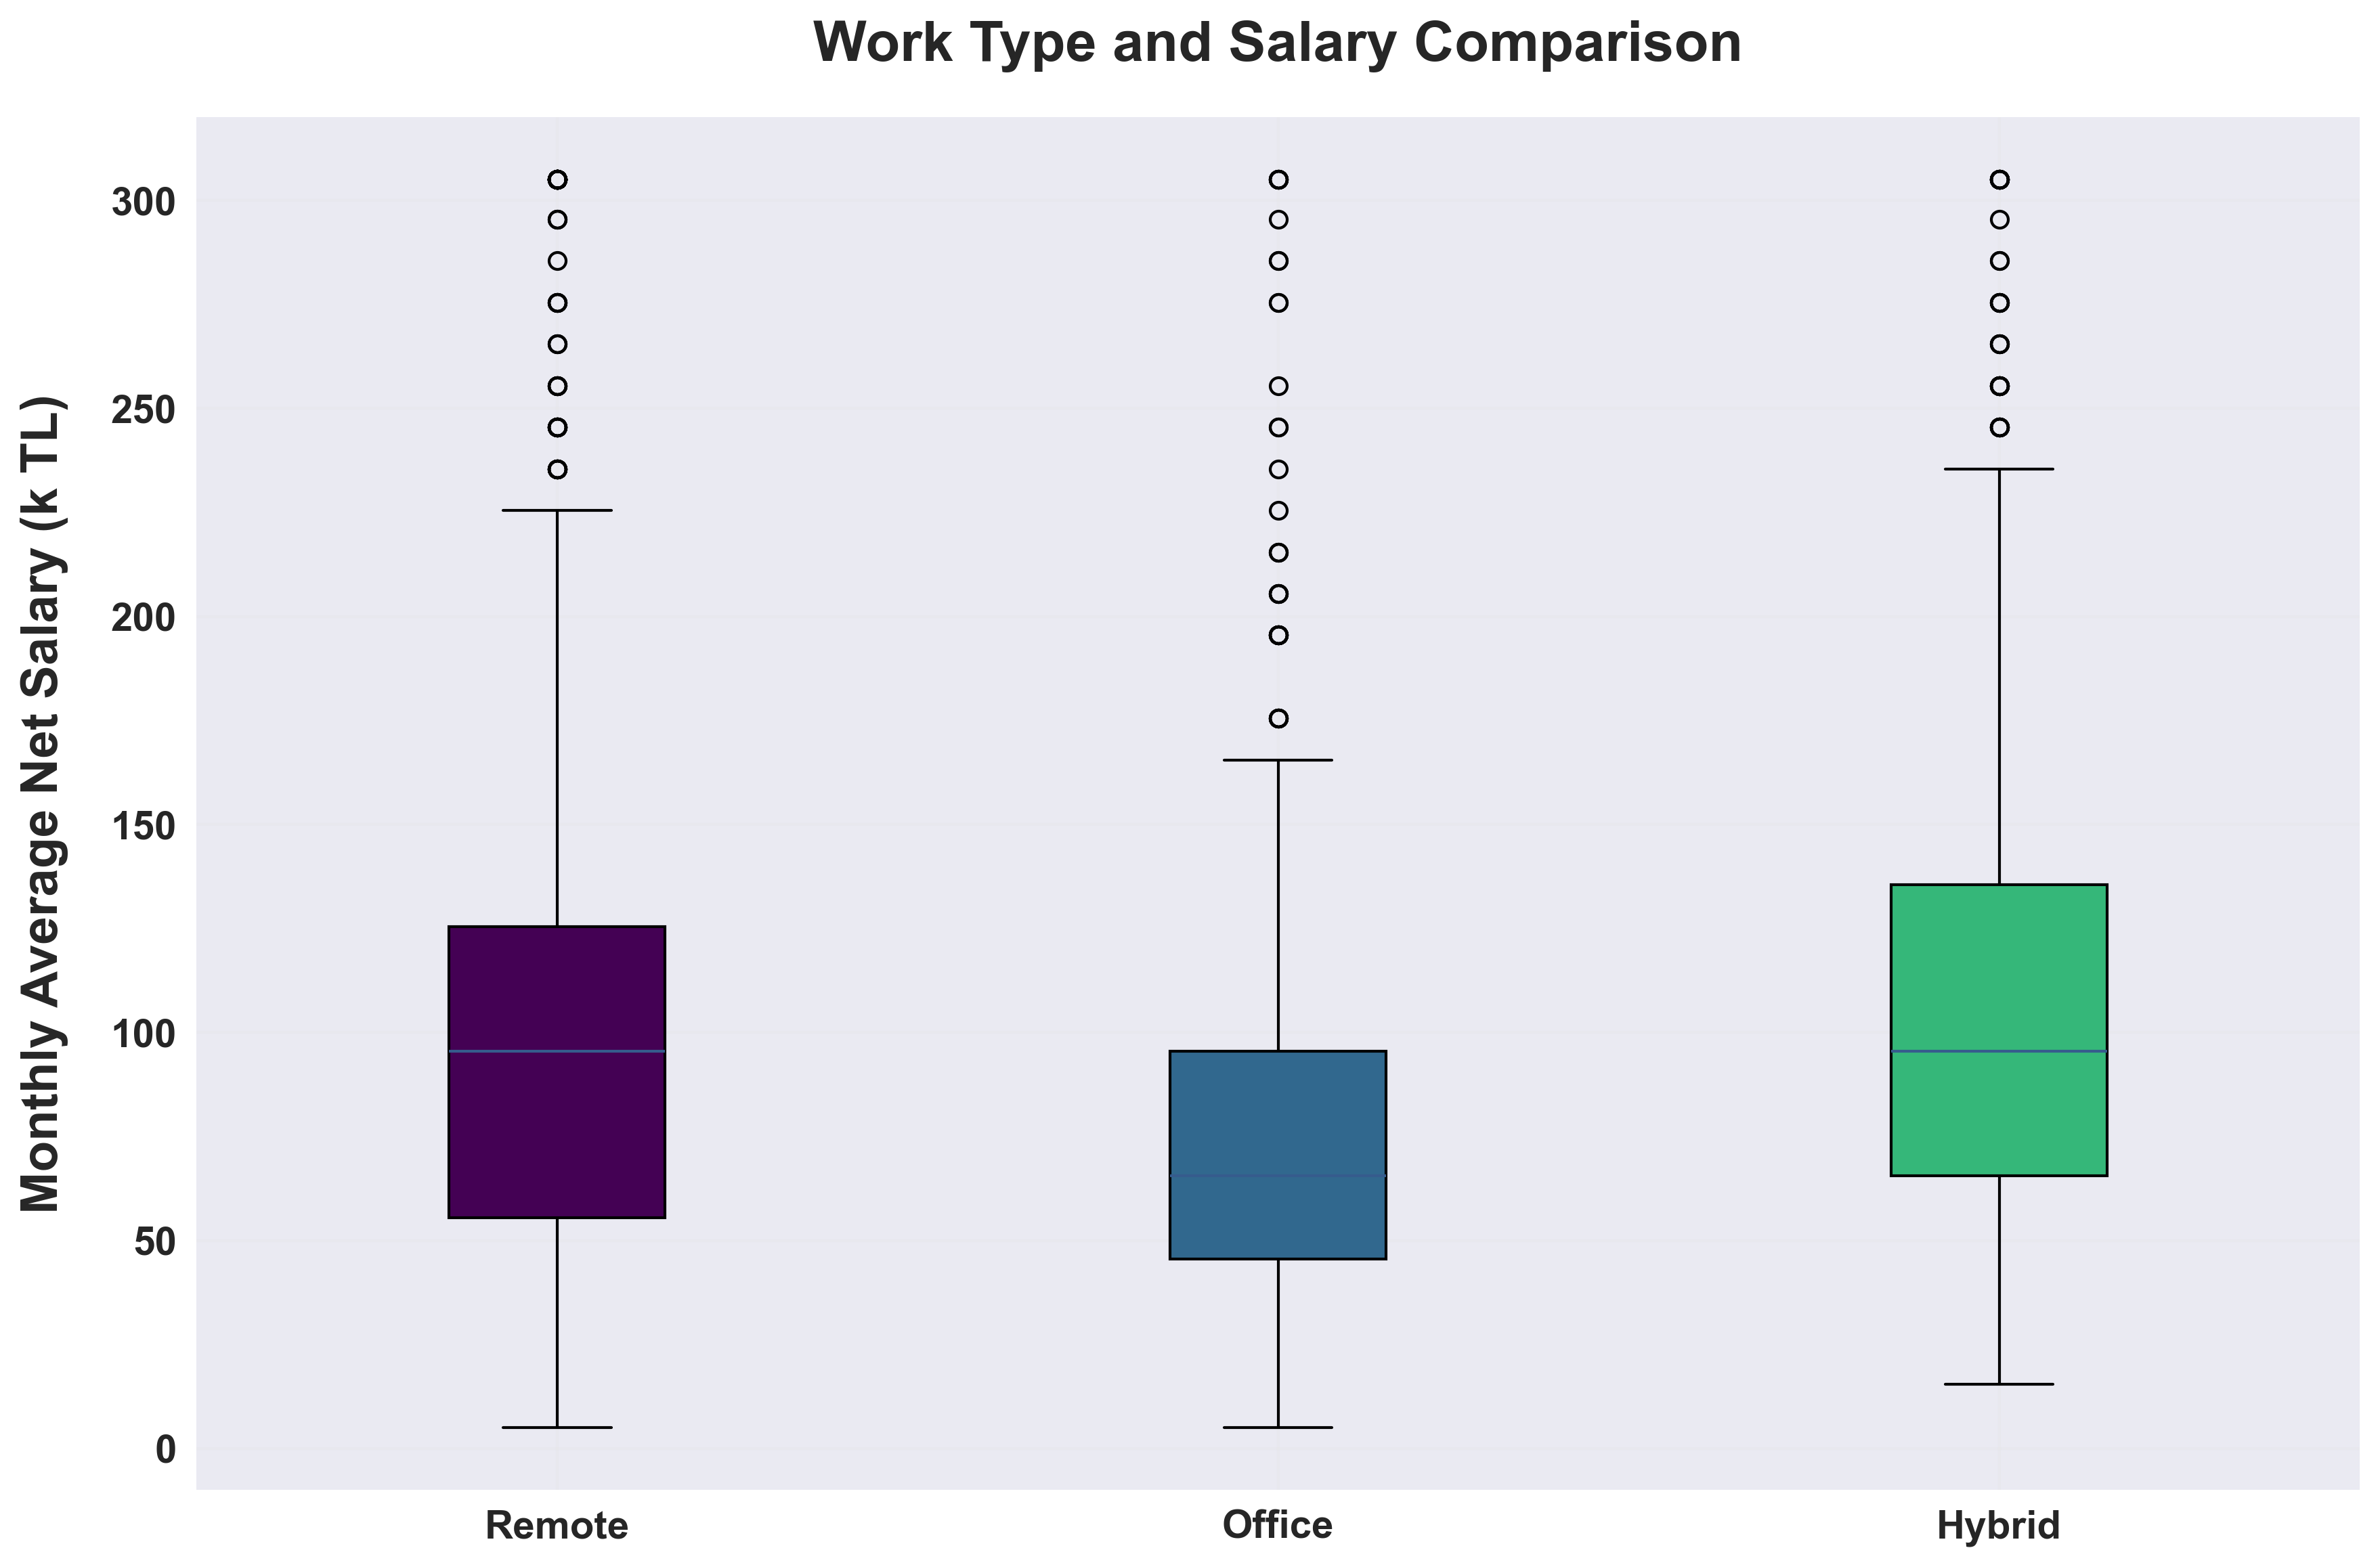
\includegraphics[width=0.85\linewidth]{figures/07_calisma_sekli_maas_karsilastirma.png}
  \caption{Salary by work arrangement (remote, office, hybrid).}
  \label{fig:work-type}
\end{figure}

\begin{figure}[H]
  \centering
  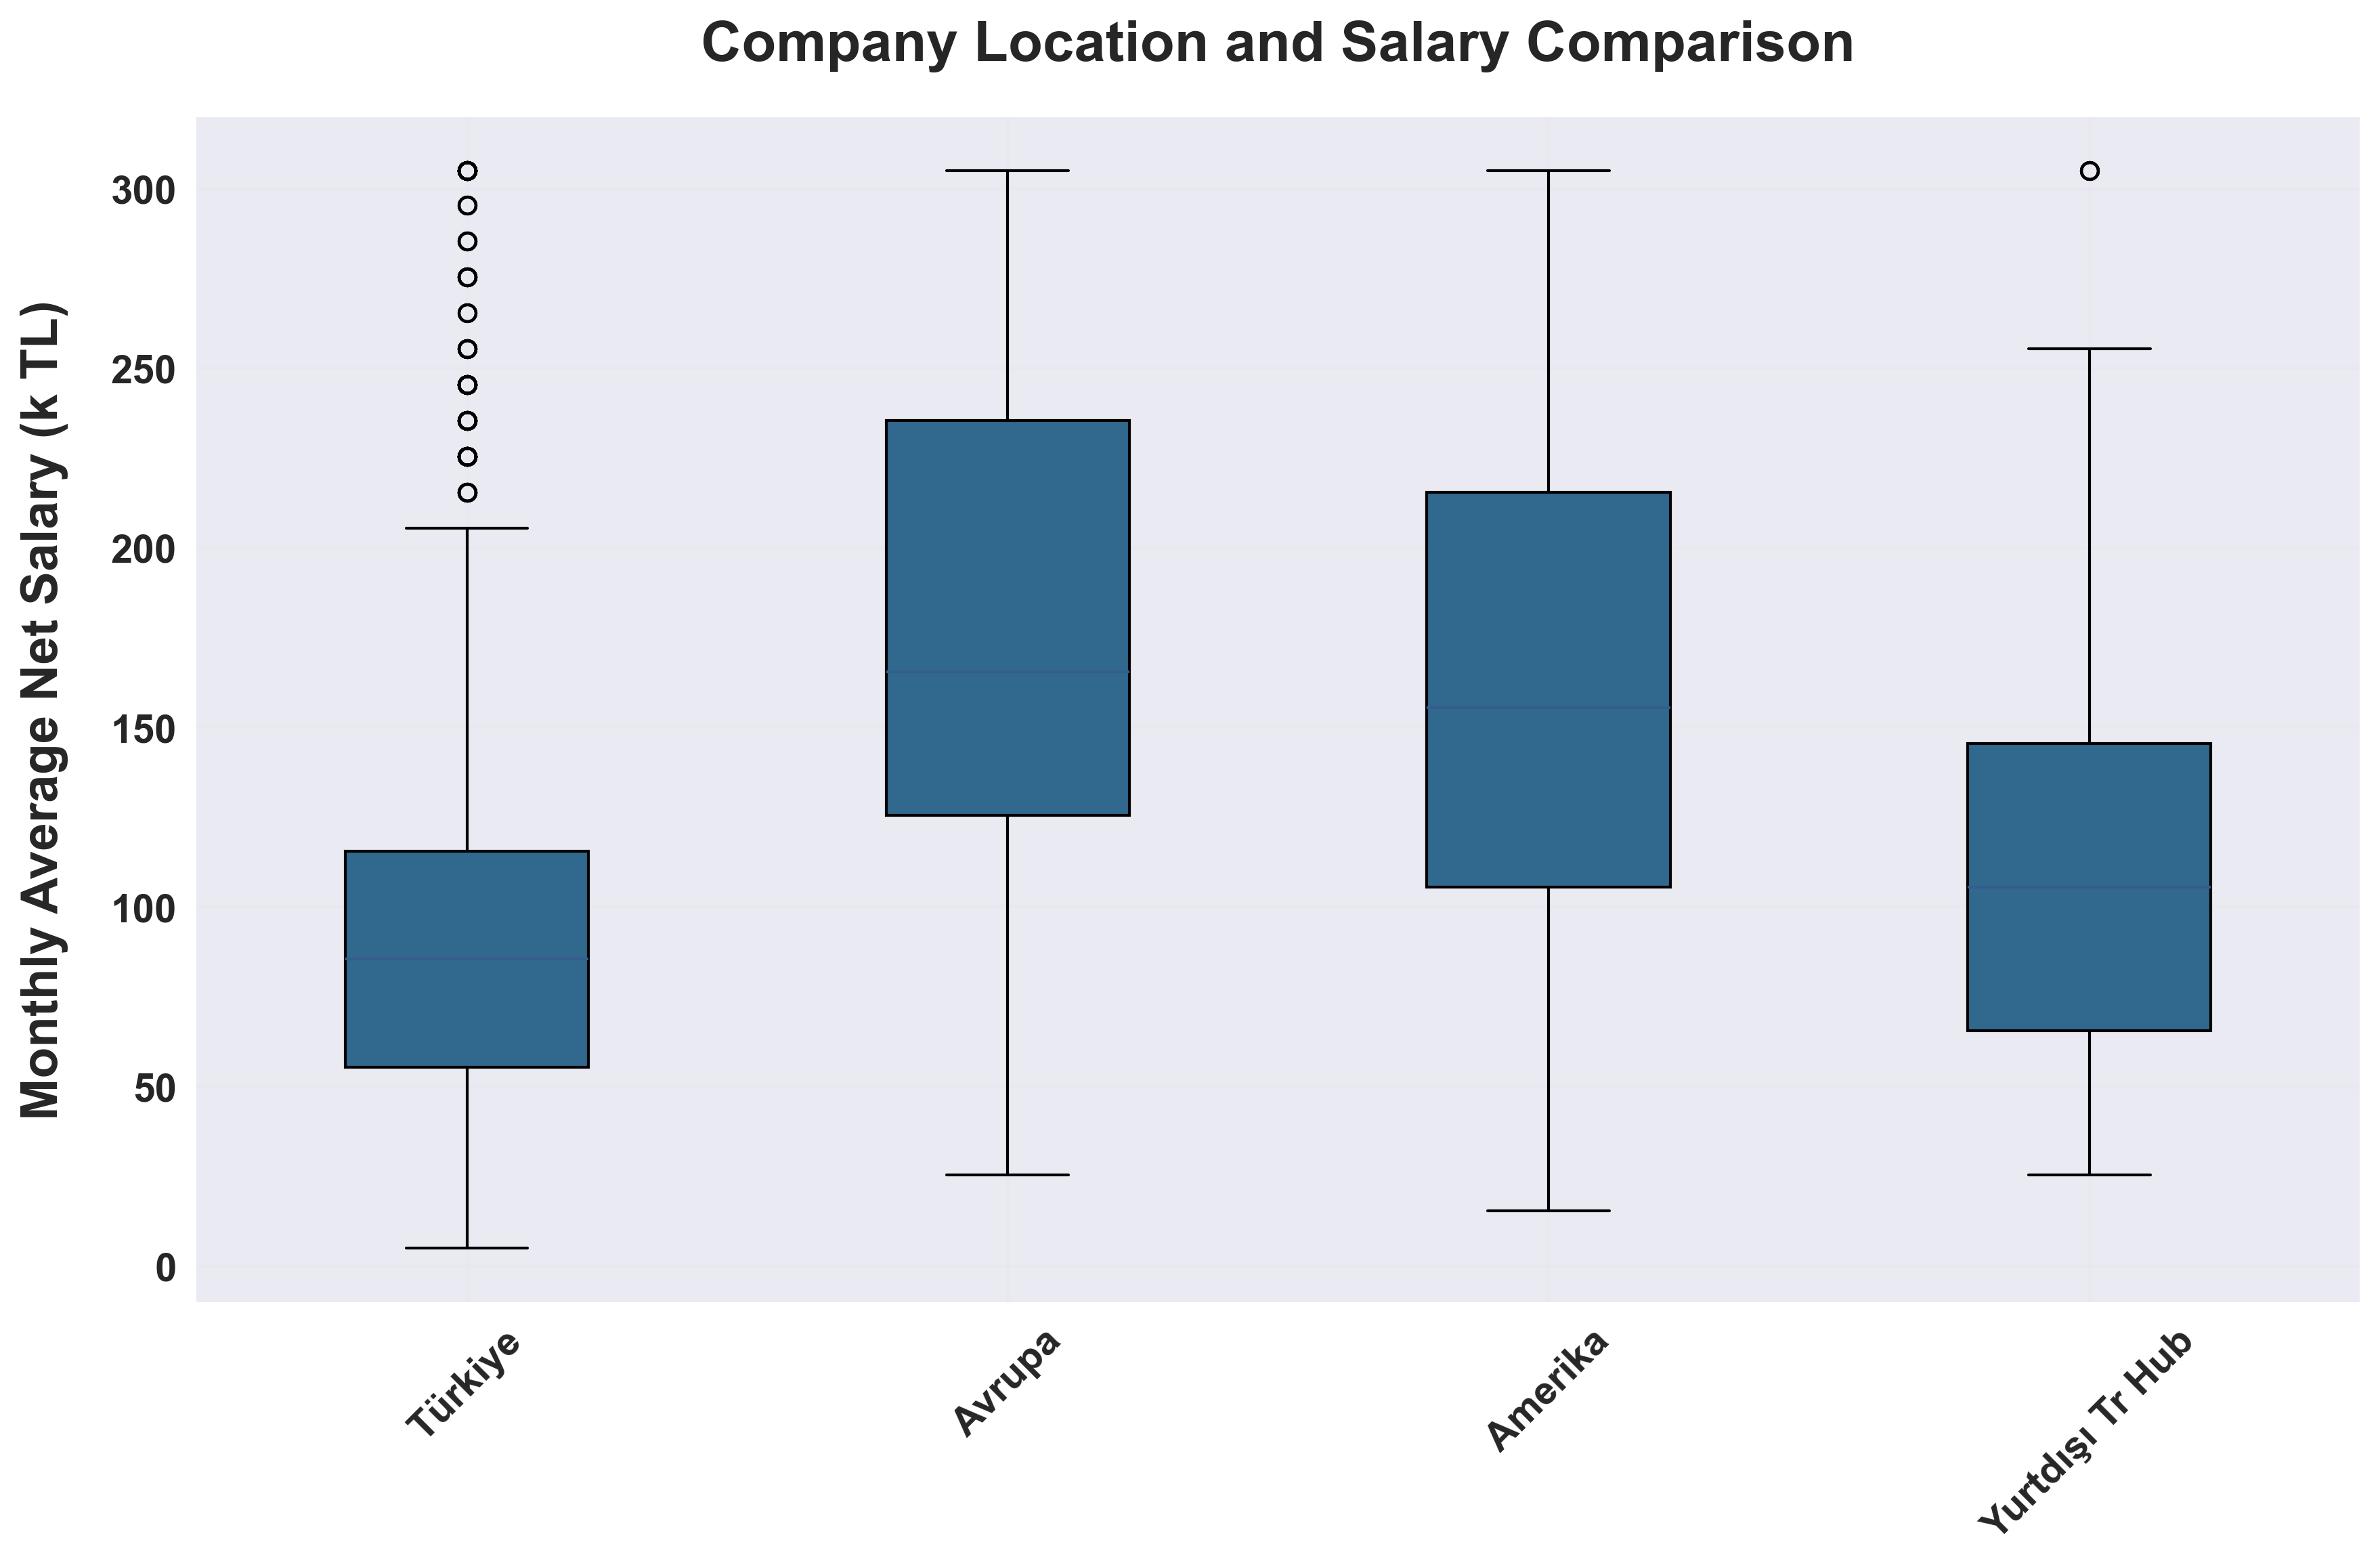
\includegraphics[width=0.85\linewidth]{figures/08_sirket_lokasyonu_maas_karsilastirma.png}
  \caption{Salary by company location.}
  \label{fig:location}
\end{figure}

\begin{figure}[H]
  \centering
  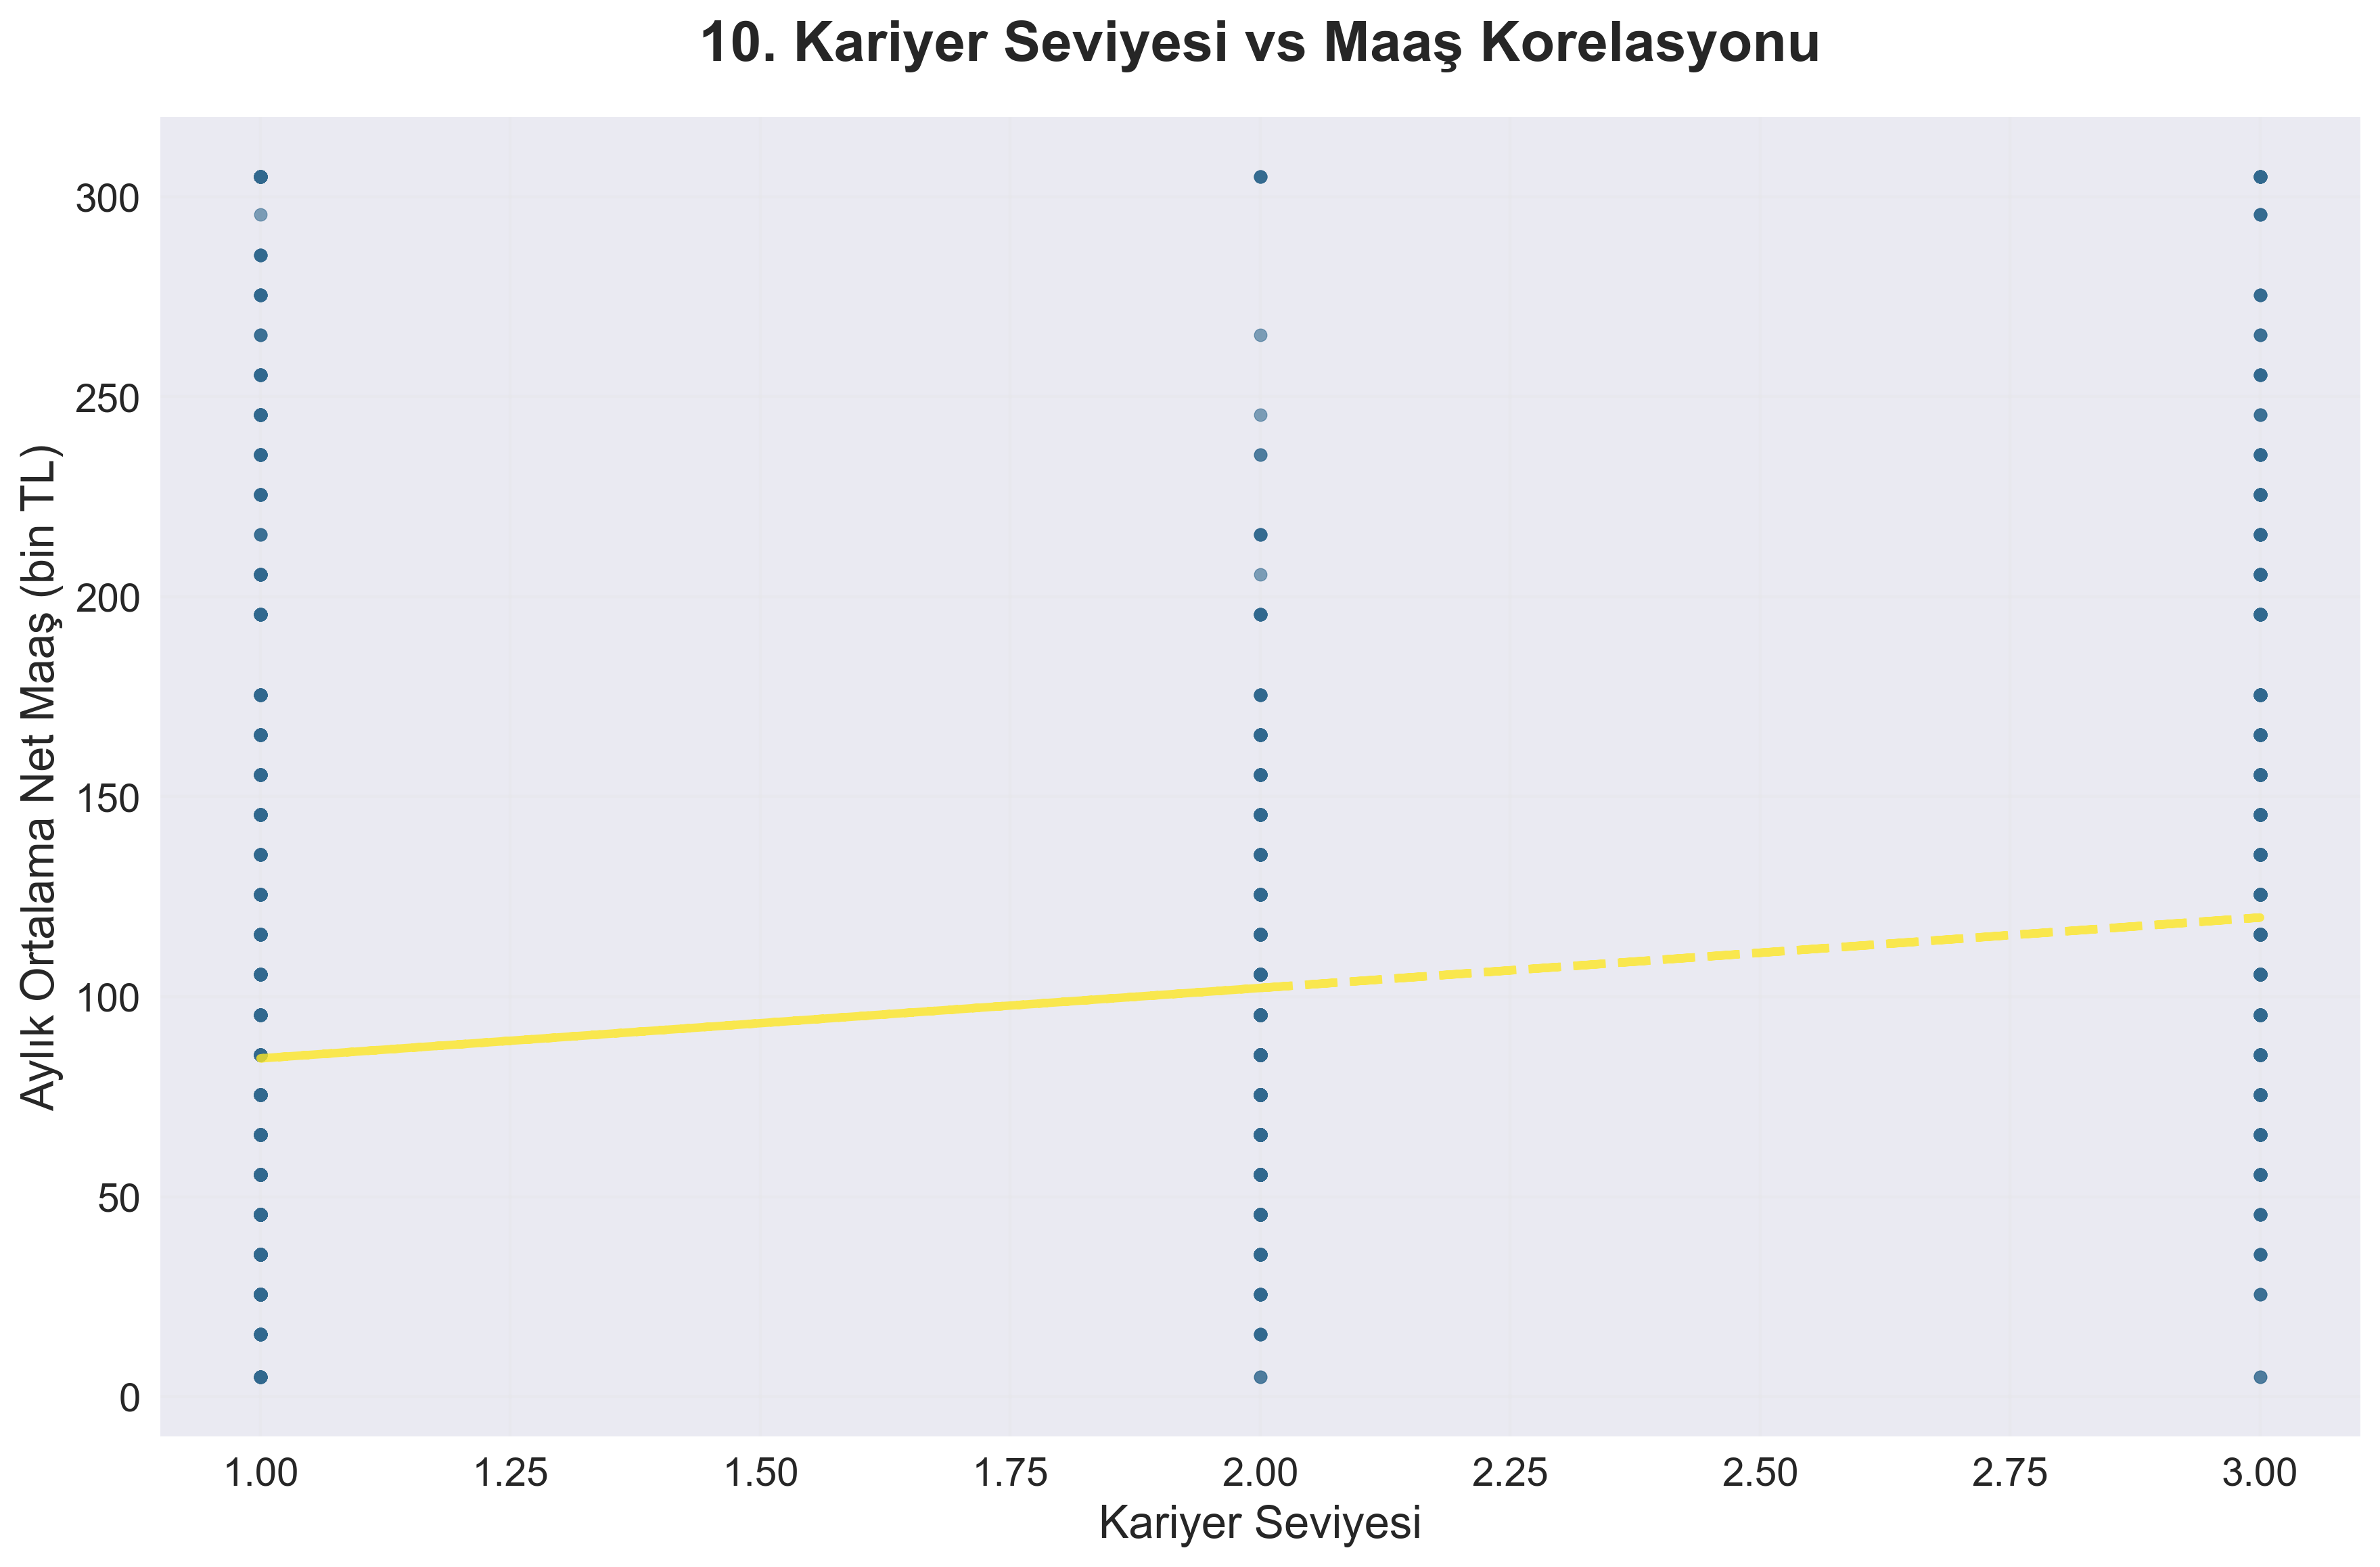
\includegraphics[width=0.85\linewidth]{figures/10_deneyim_maas_scatter.png}
  \caption{Experience vs salary (scatter).}
  \label{fig:experience}
\end{figure}

% New engaging figures
\begin{figure}[H]
  \centering
  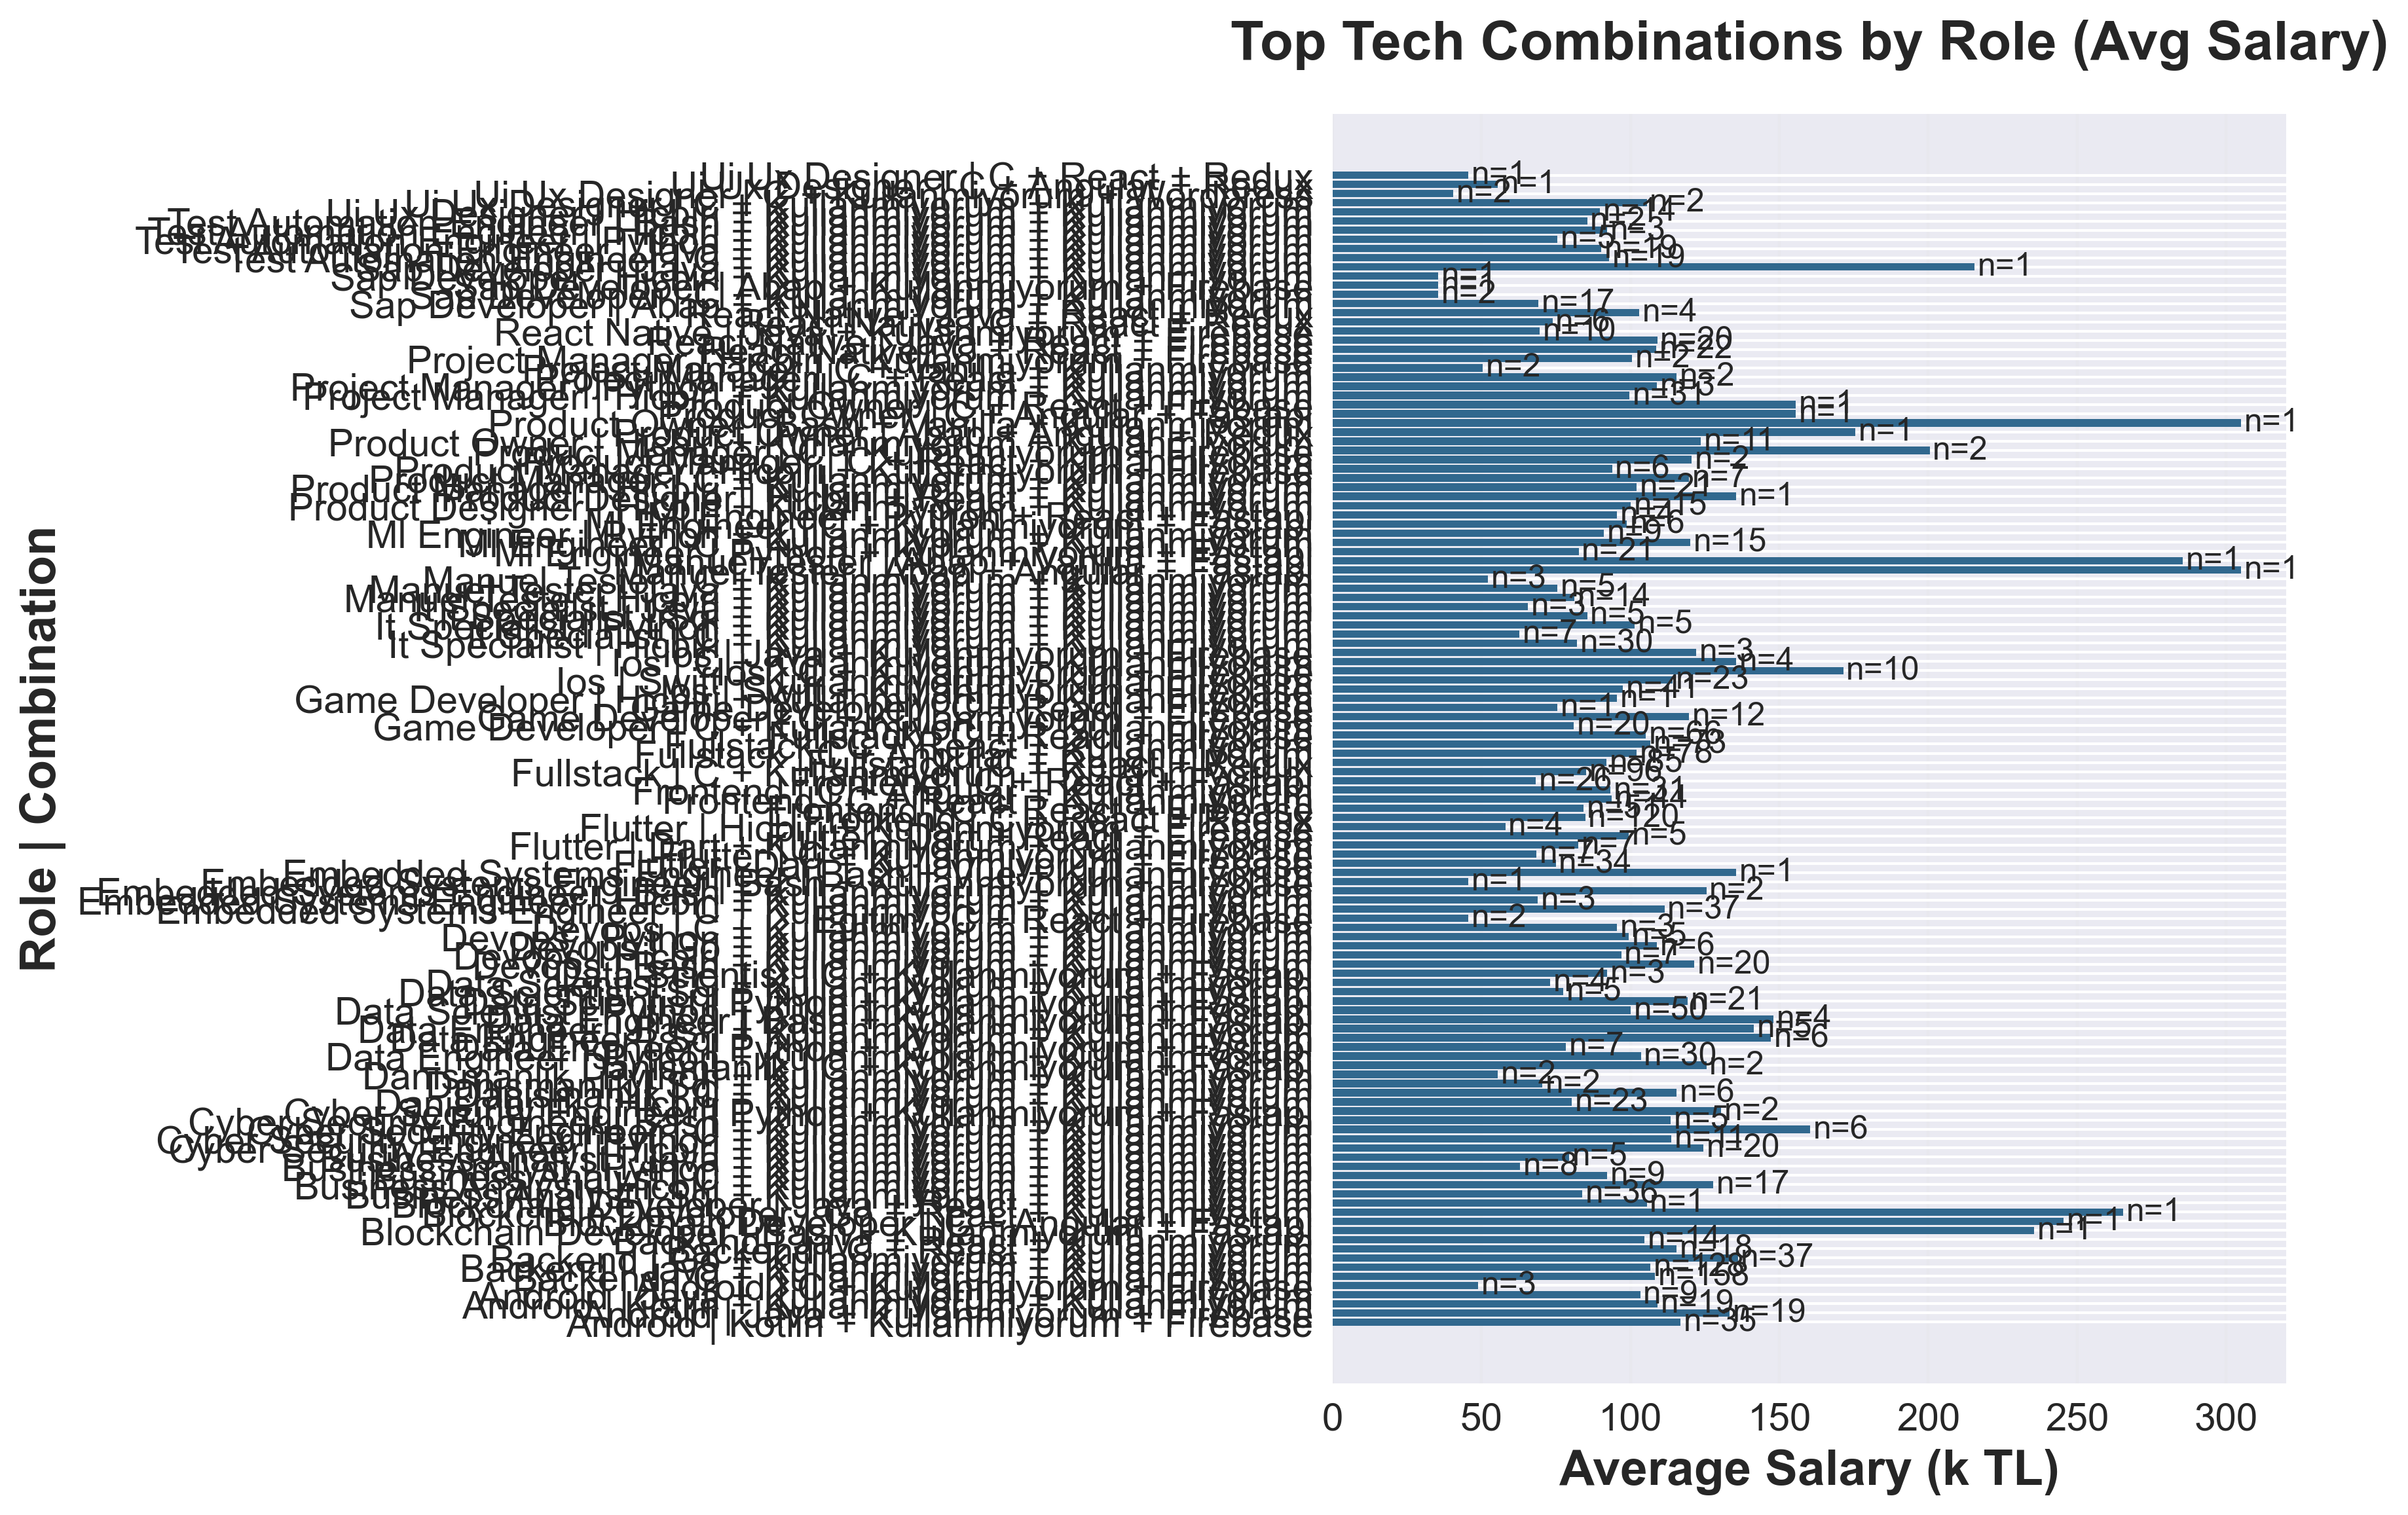
\includegraphics[width=0.85\linewidth]{figures/21_tech_combo_top.png}
  \caption{Top tech combinations by role with average salaries.}
  \label{fig:tech-combos}
\end{figure}

\begin{figure}[H]
  \centering
  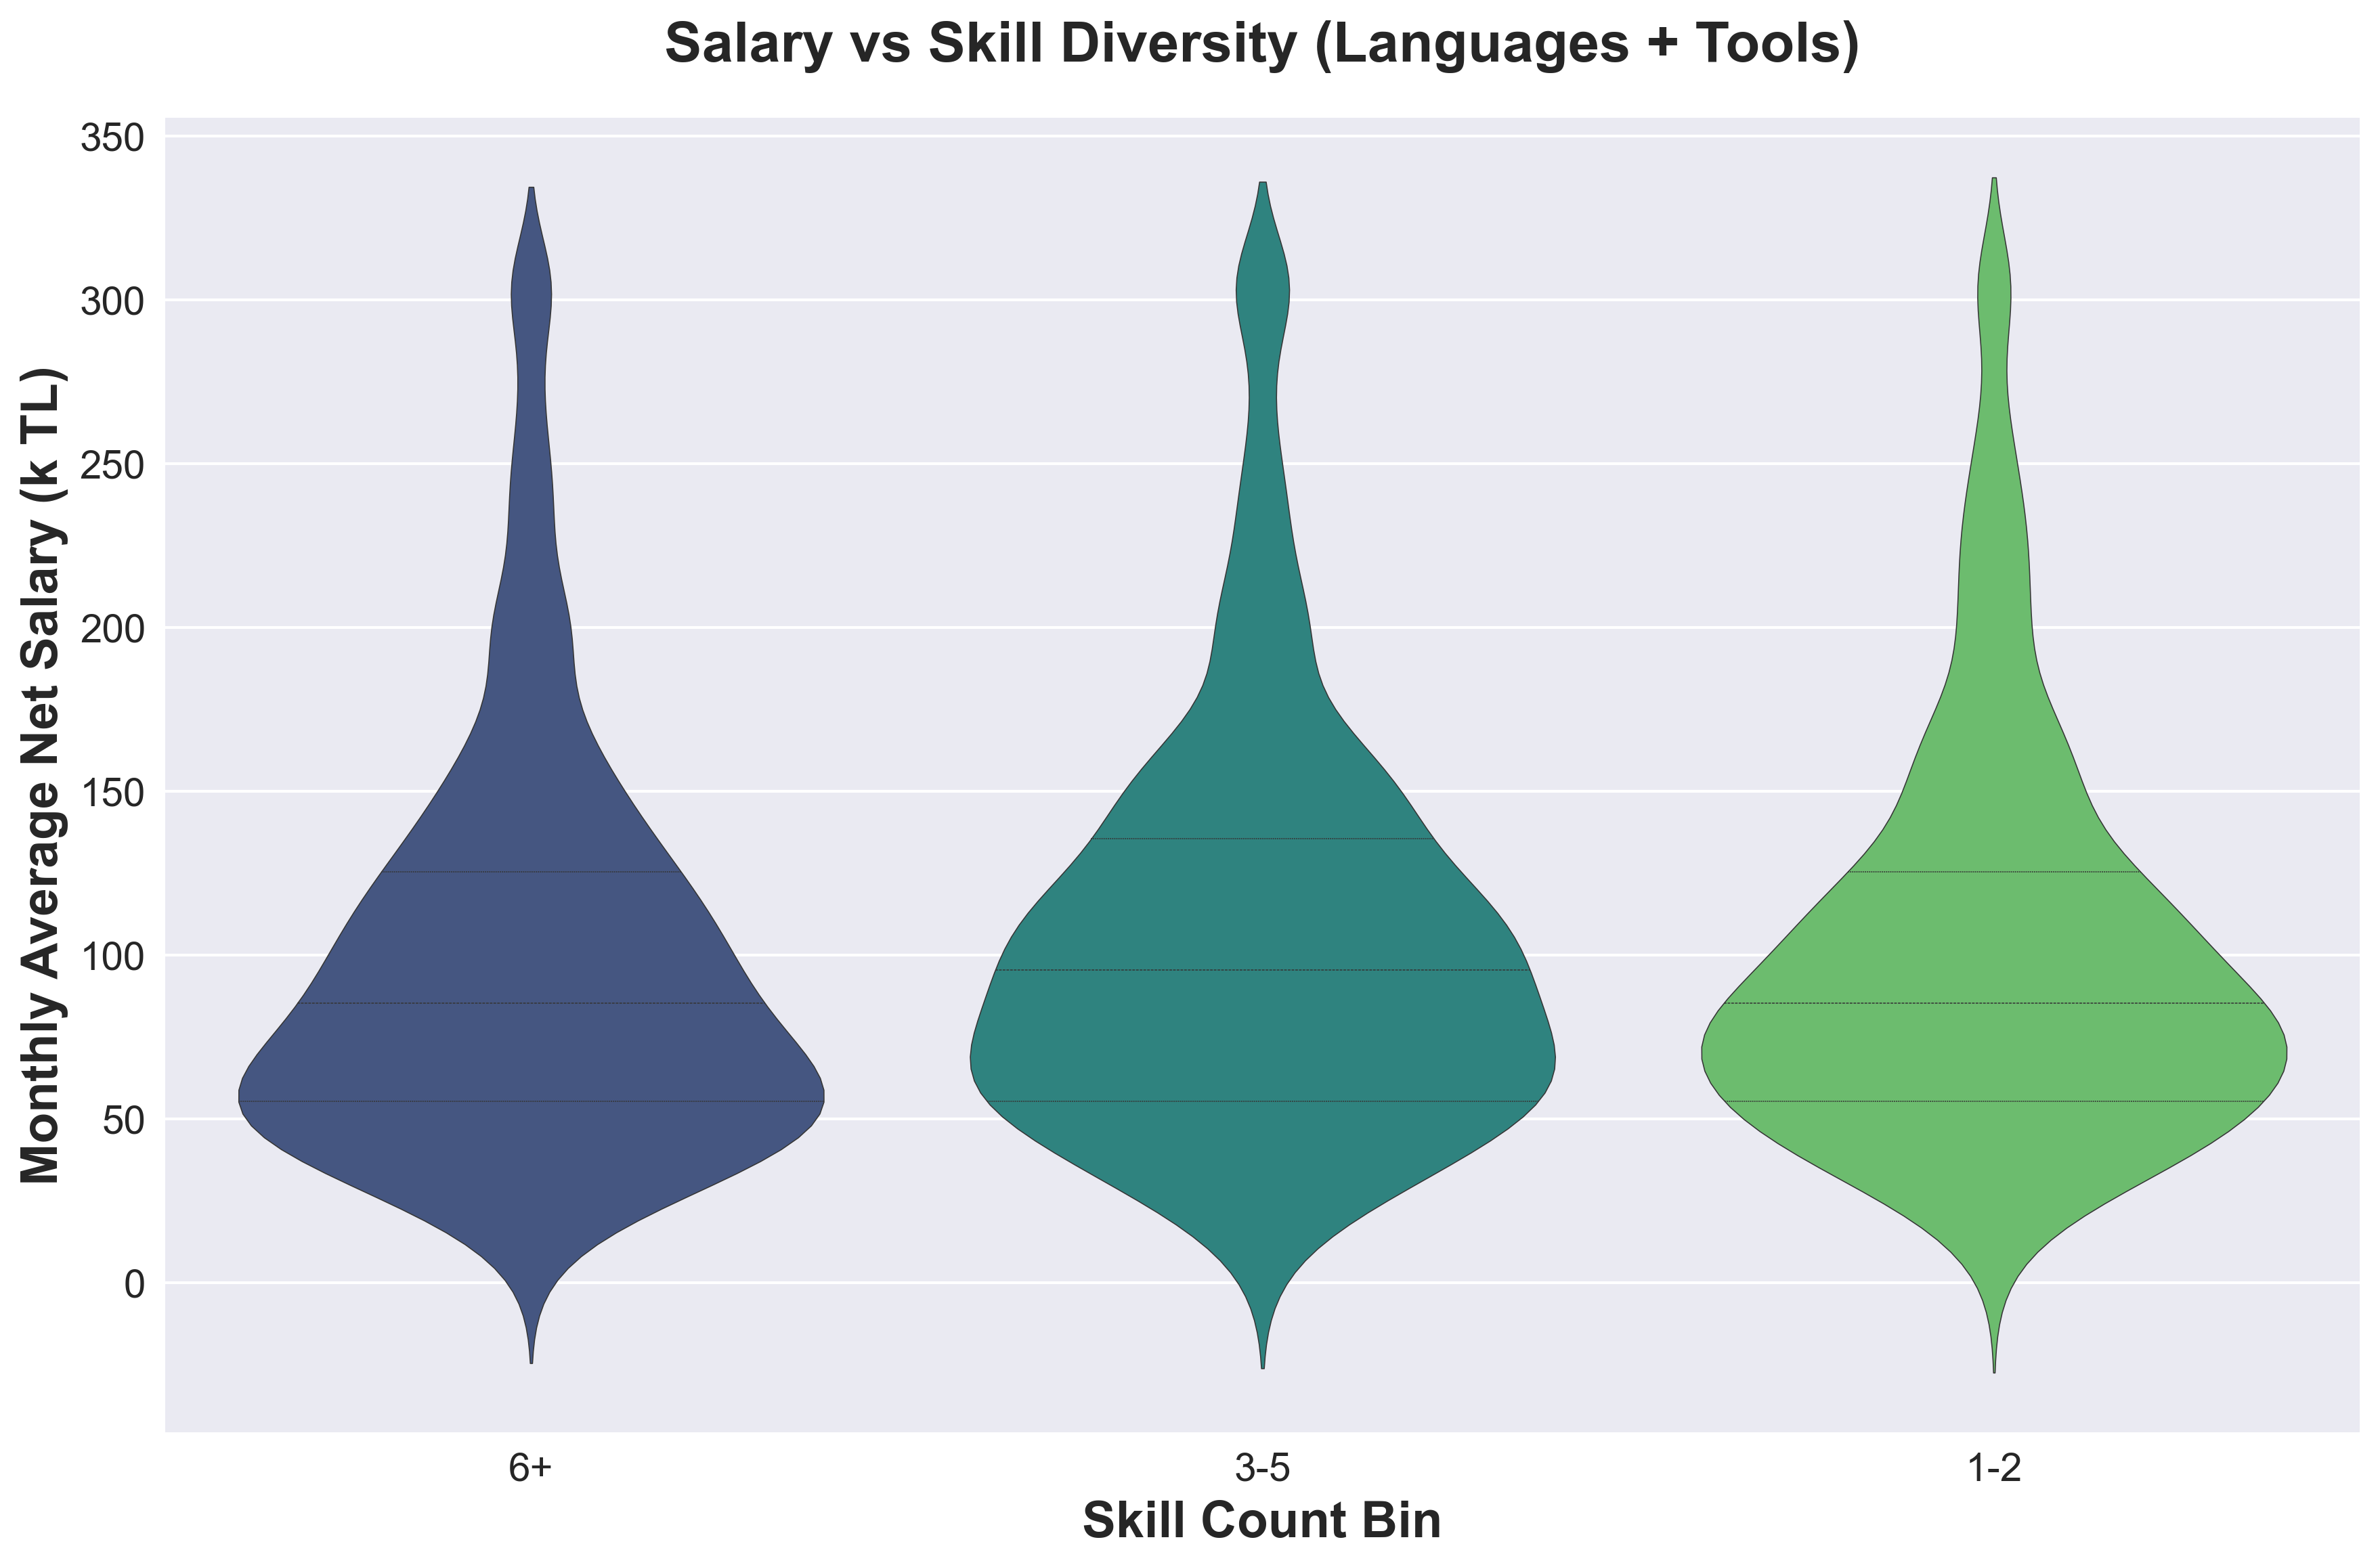
\includegraphics[width=0.85\linewidth]{figures/22_skill_diversity_salary.png}
  \caption{Salary distribution by skill diversity (languages + tools).}
  \label{fig:skill-diversity}
\end{figure}

\begin{figure}[H]
  \centering
  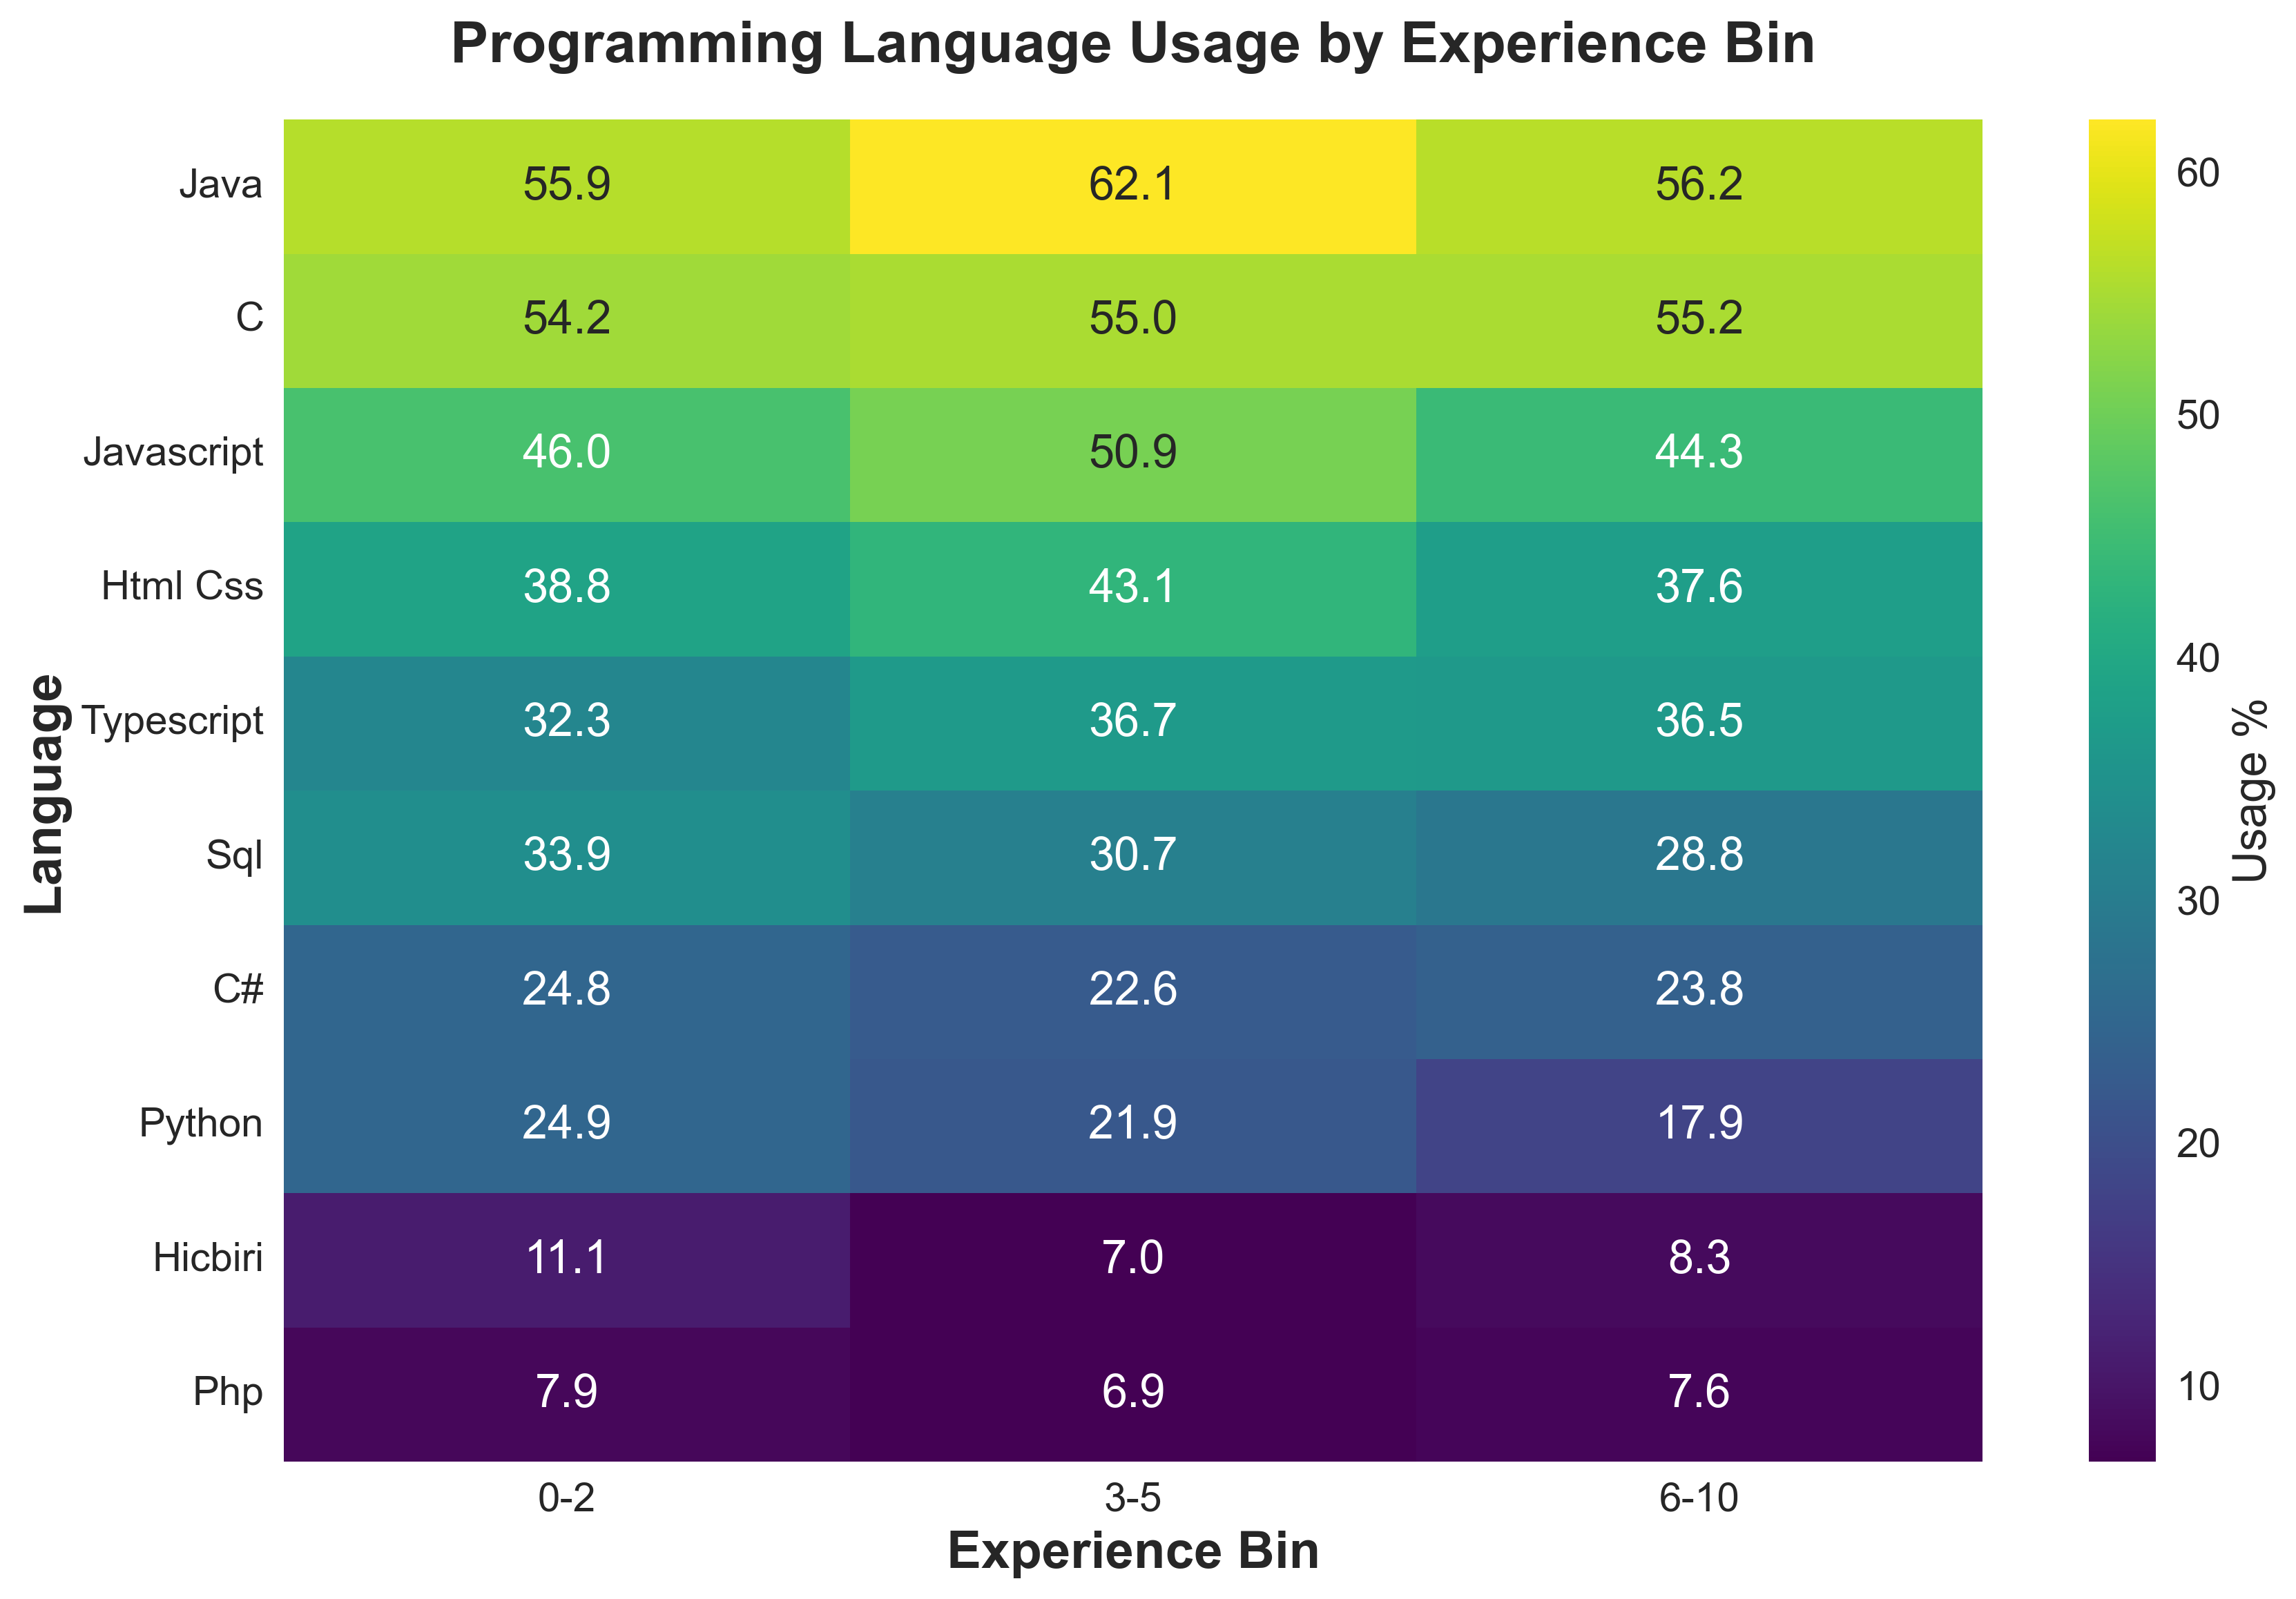
\includegraphics[width=0.85\linewidth]{figures/23_experience_lang_usage_heatmap.png}
  \caption{Programming language usage by experience bin.}
  \label{fig:exp-usage}
\end{figure}

\begin{figure}[H]
  \centering
  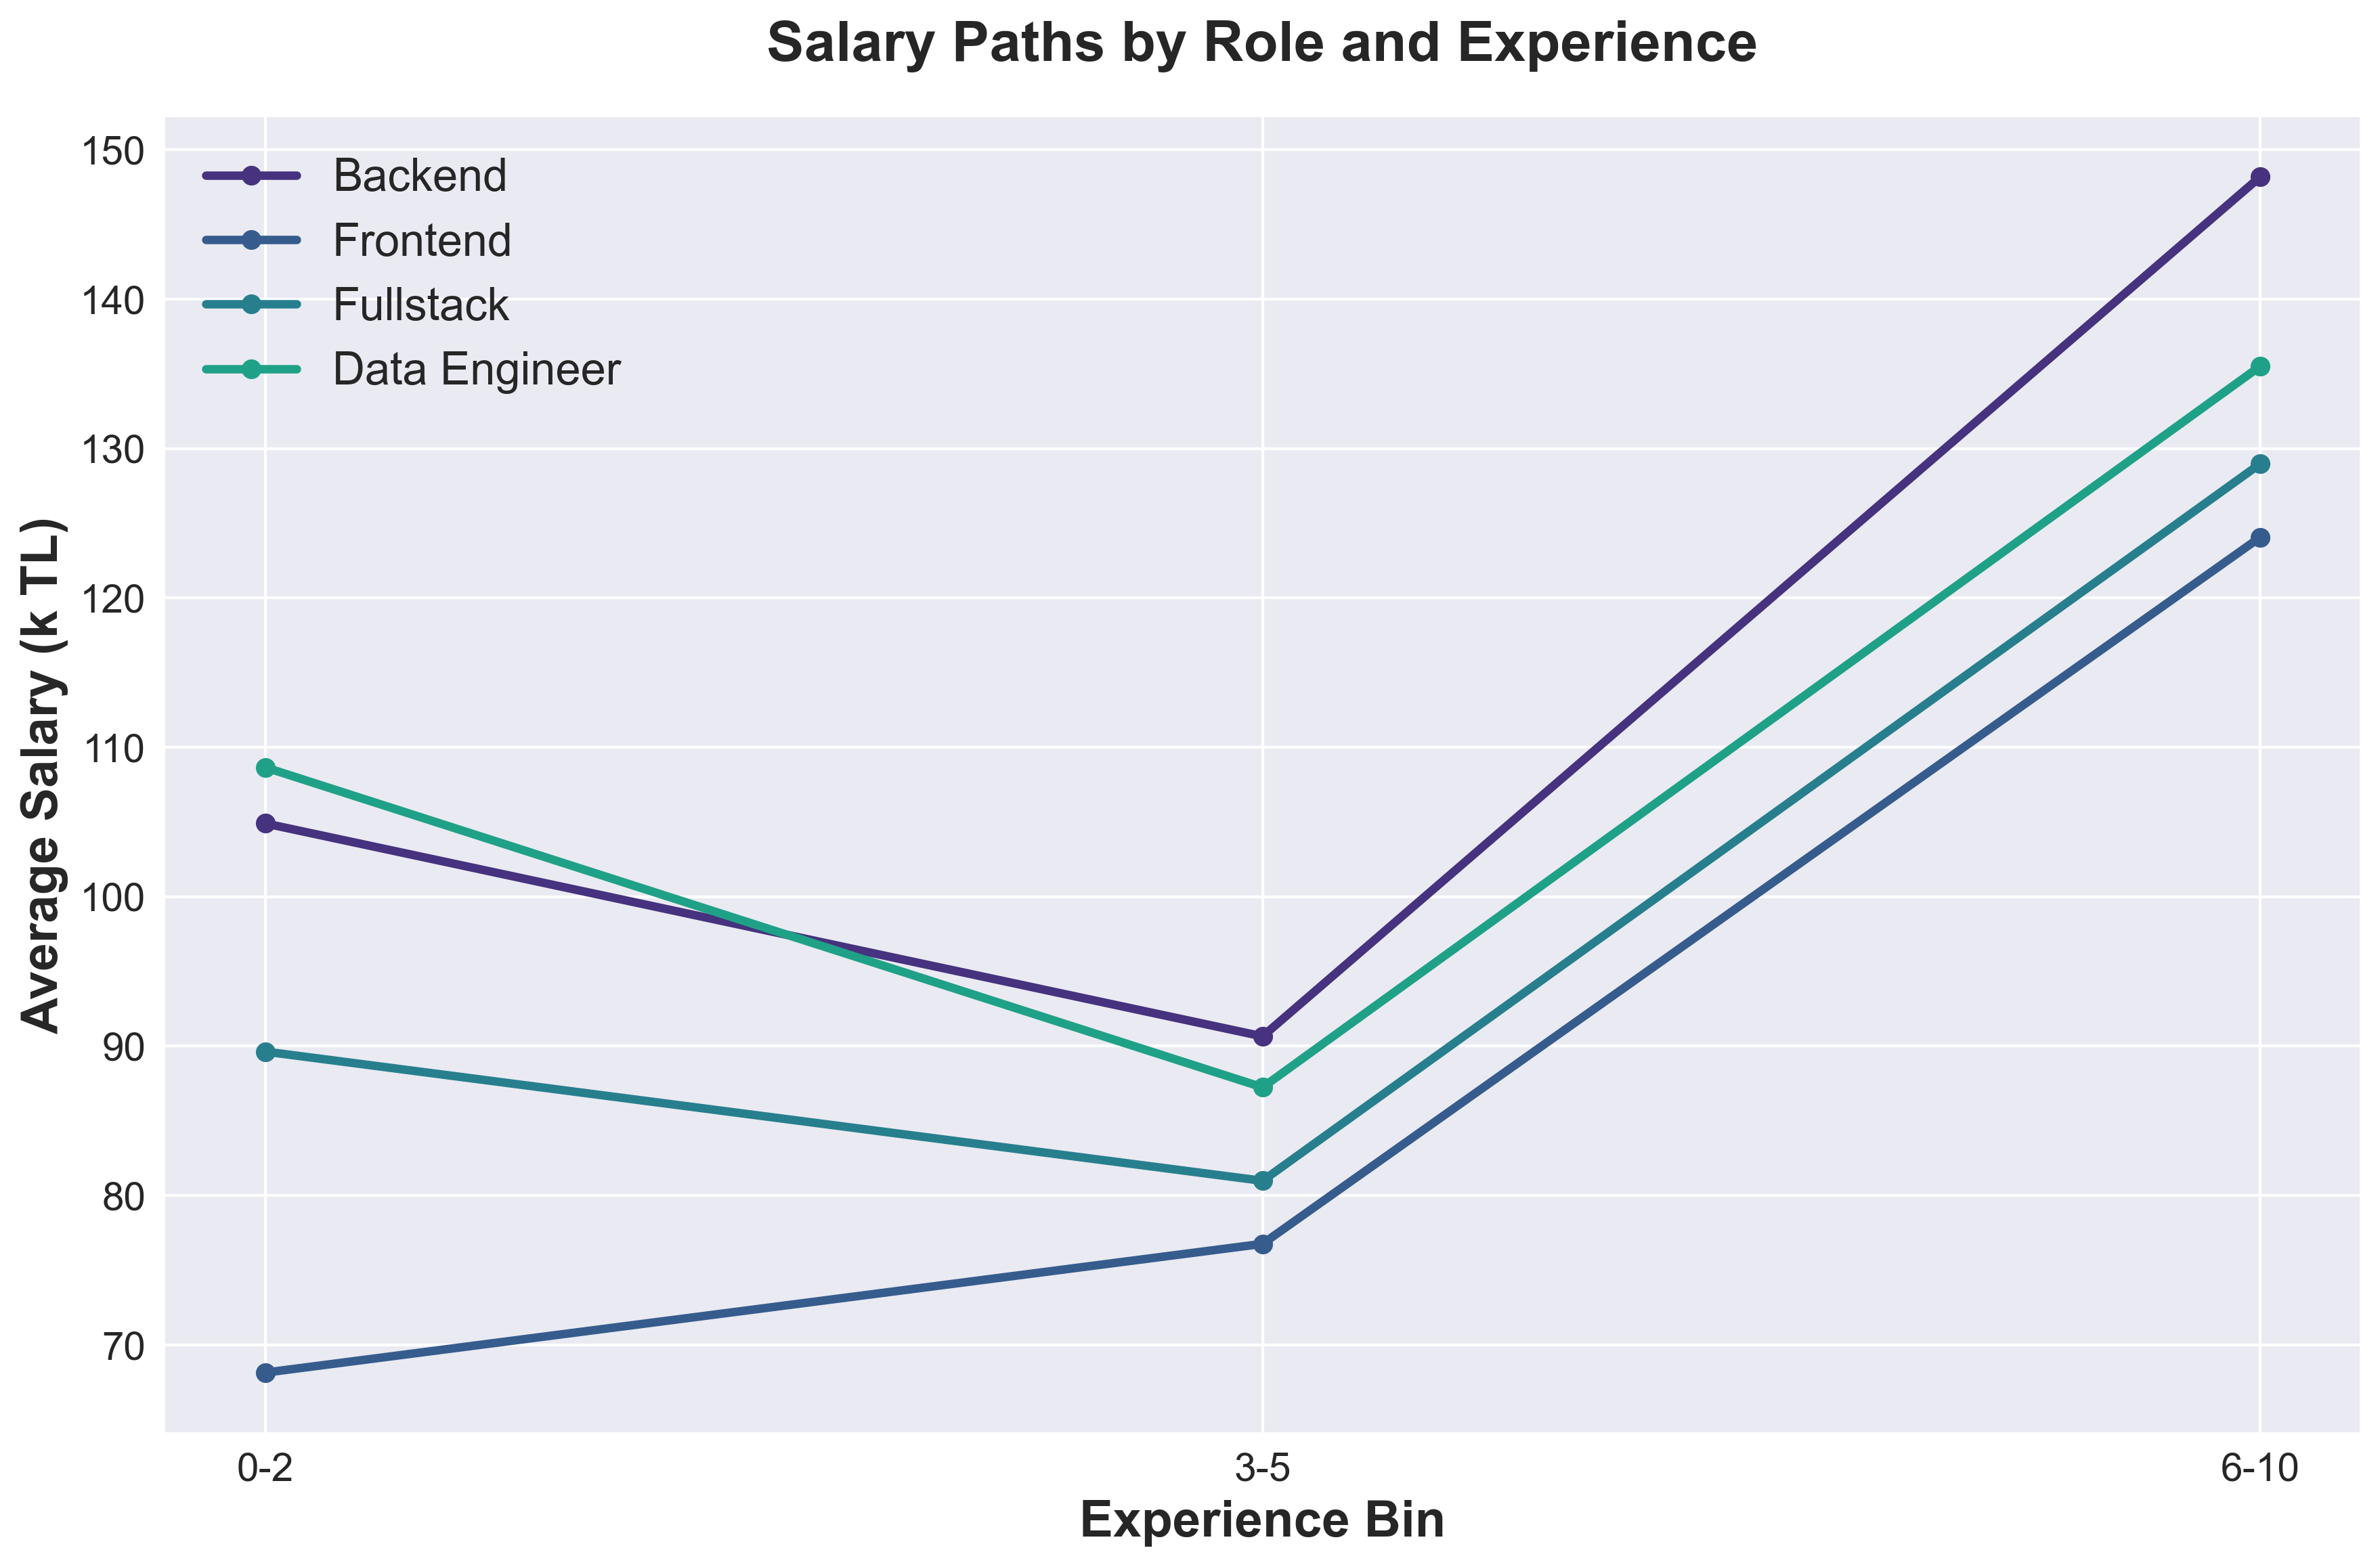
\includegraphics[width=0.85\linewidth]{figures/24_role_experience_salary_paths.png}
  \caption{Salary paths by role and experience.}
  \label{fig:role-exp-salary}
\end{figure}

\begin{figure}[H]
  \centering
  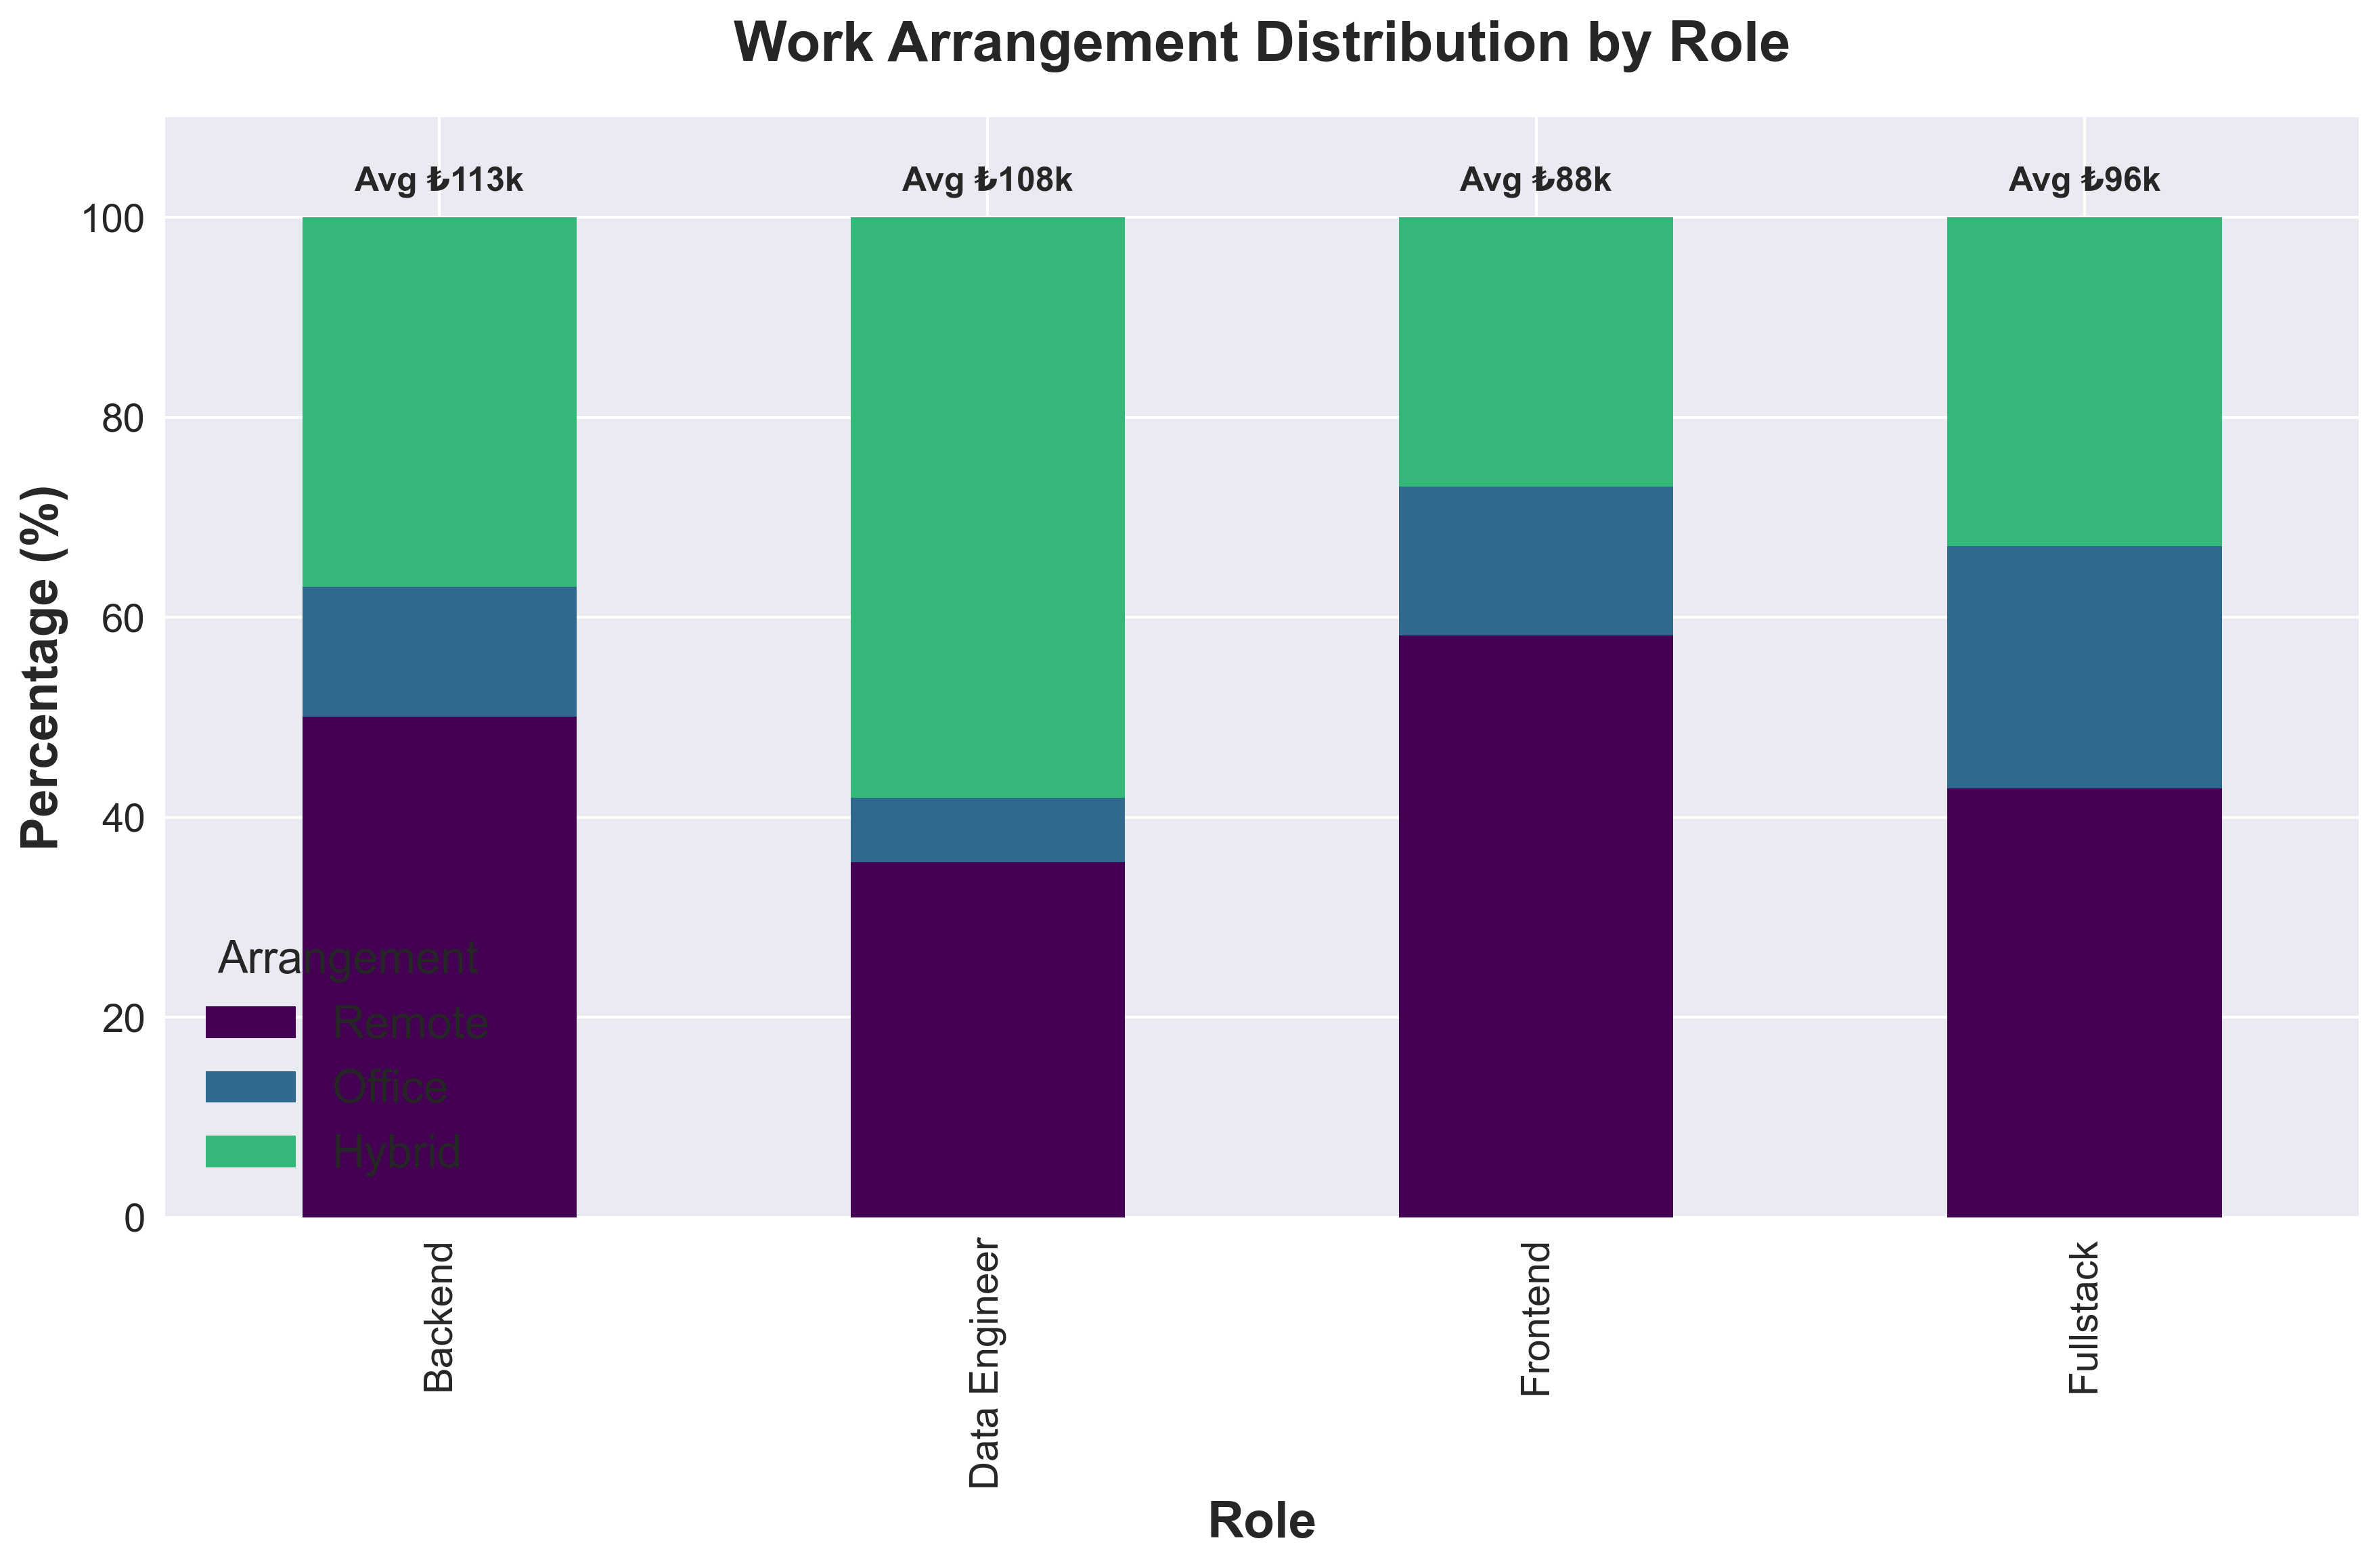
\includegraphics[width=0.85\linewidth]{figures/26_work_arrangement_by_role.png}
  \caption{Work arrangement distribution by role with average salary annotations.}
  \label{fig:work-arrangement-role}
\end{figure}

\begin{figure}[H]
  \centering
  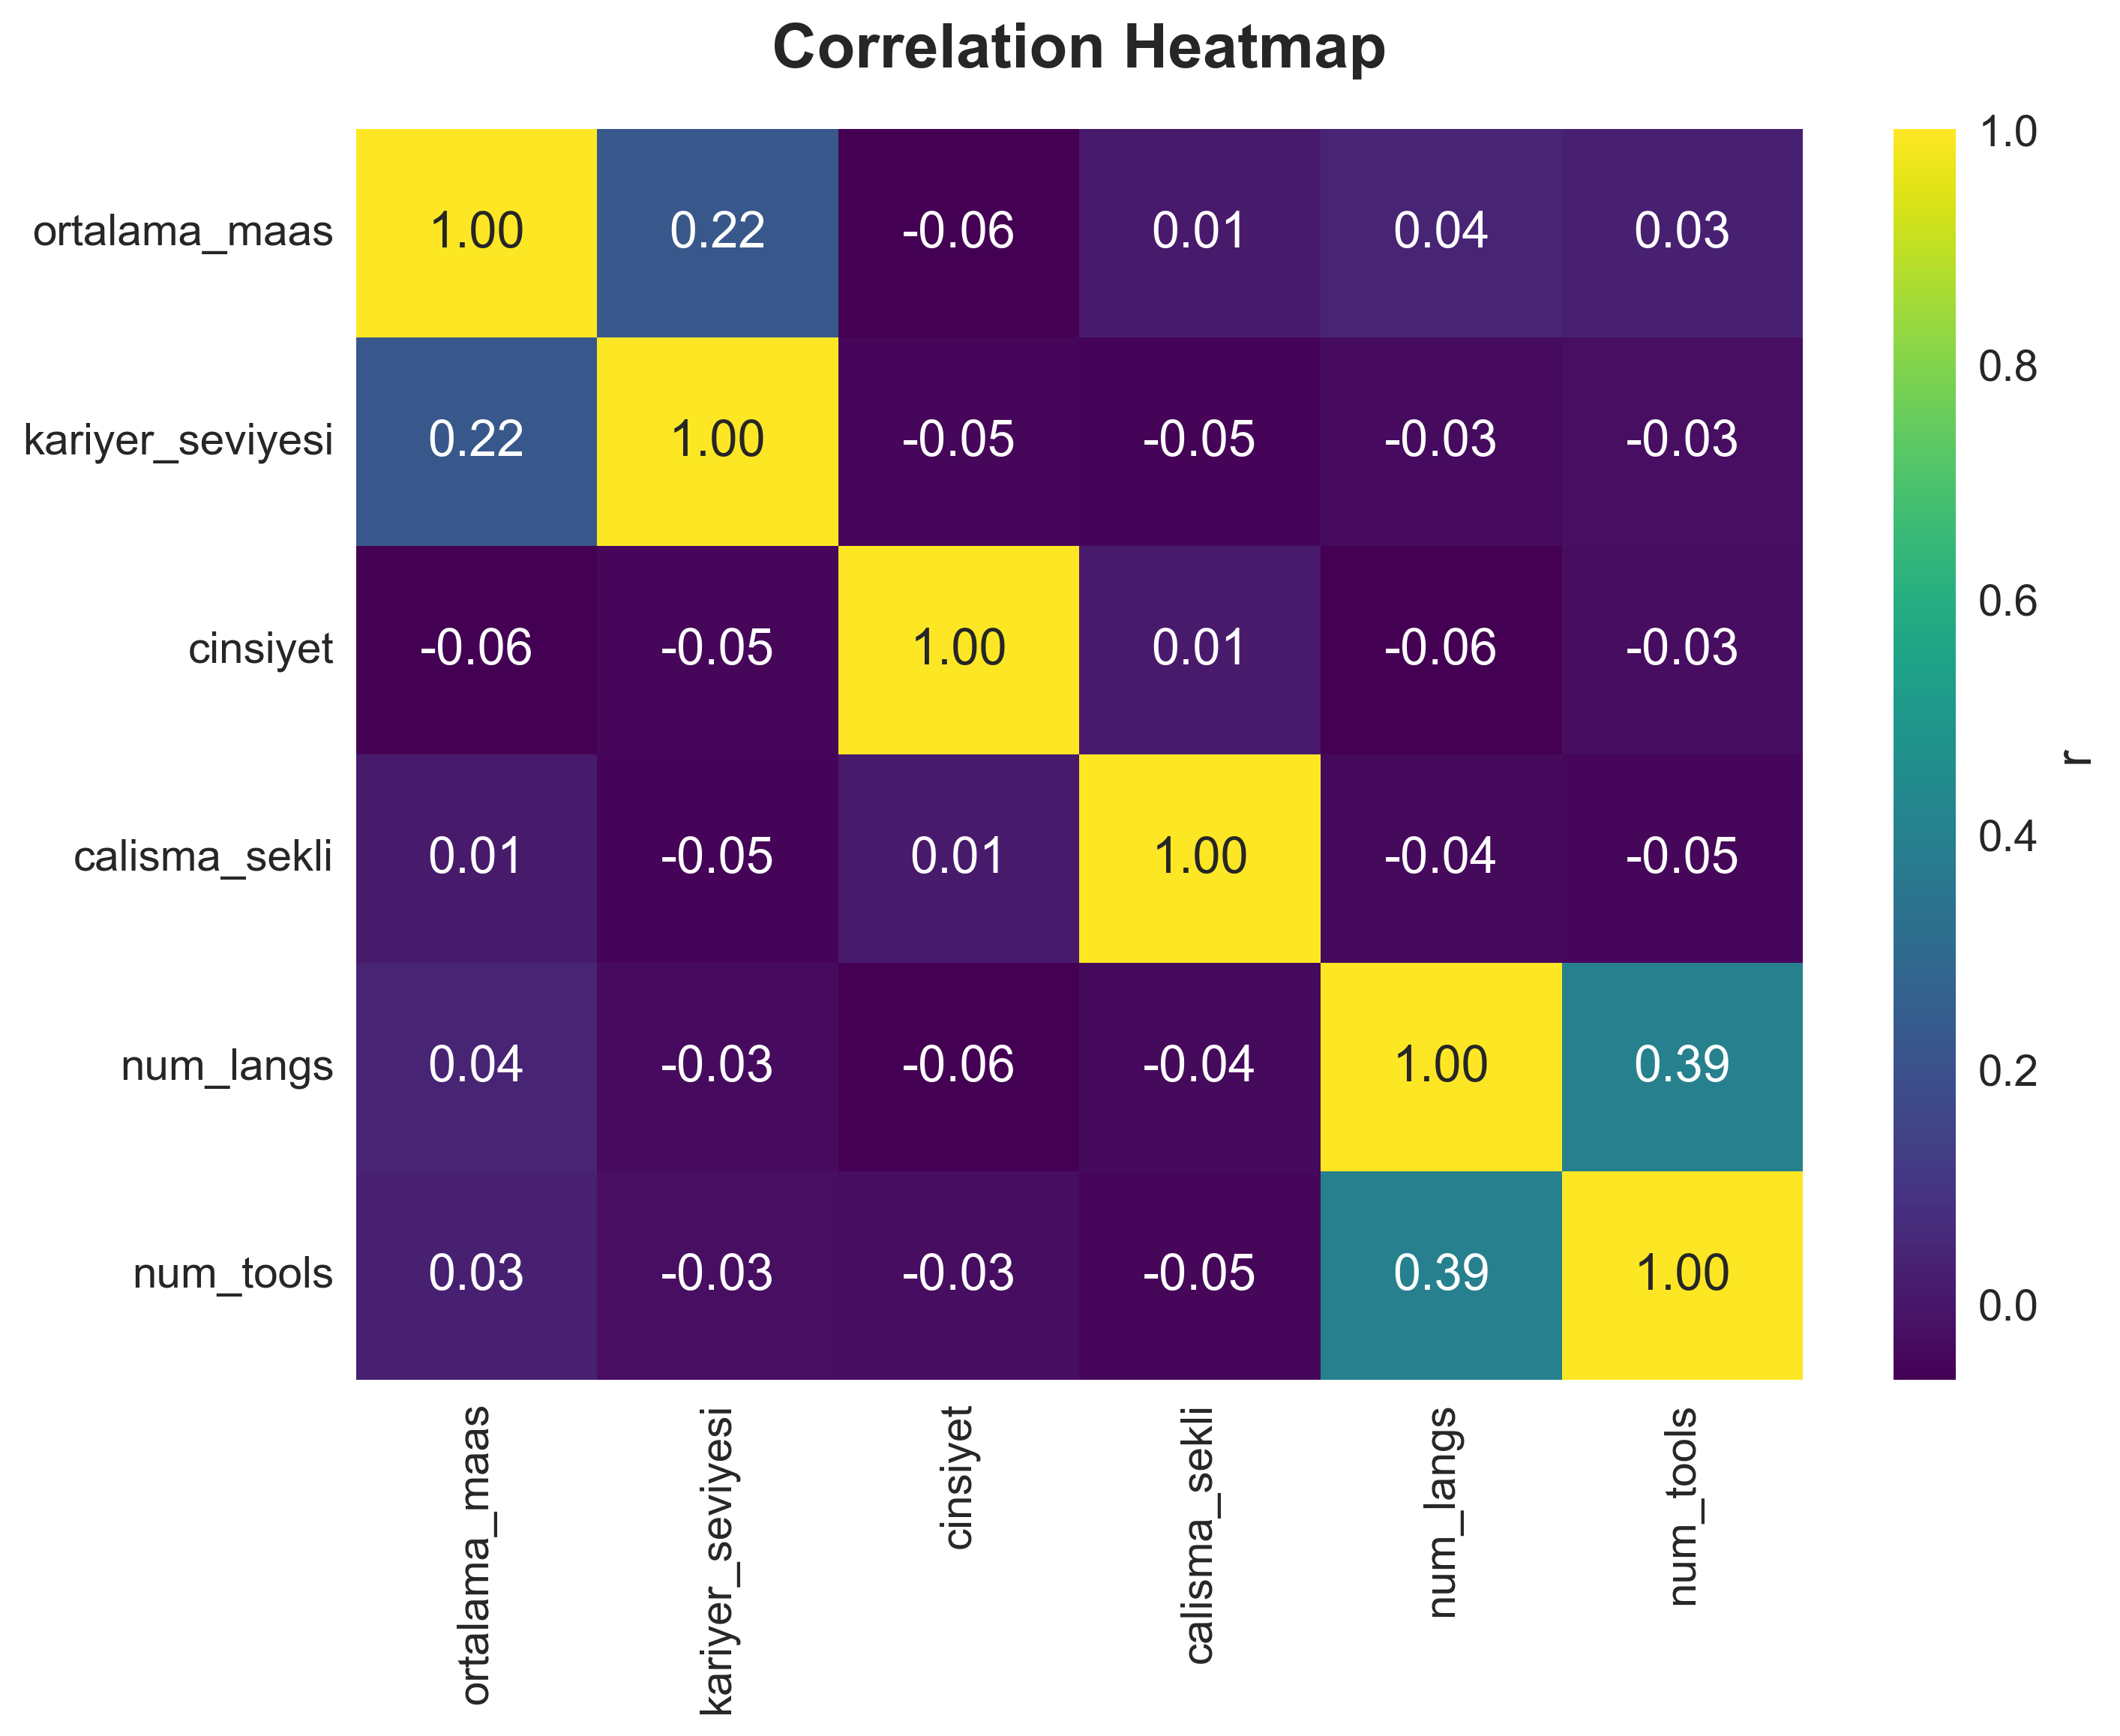
\includegraphics[width=0.85\linewidth]{figures/27_correlation_heatmap.png}
  \caption{Correlation heatmap across selected variables.}
  \label{fig:corr-heatmap}
\end{figure}

\begin{figure}[H]
  \centering
  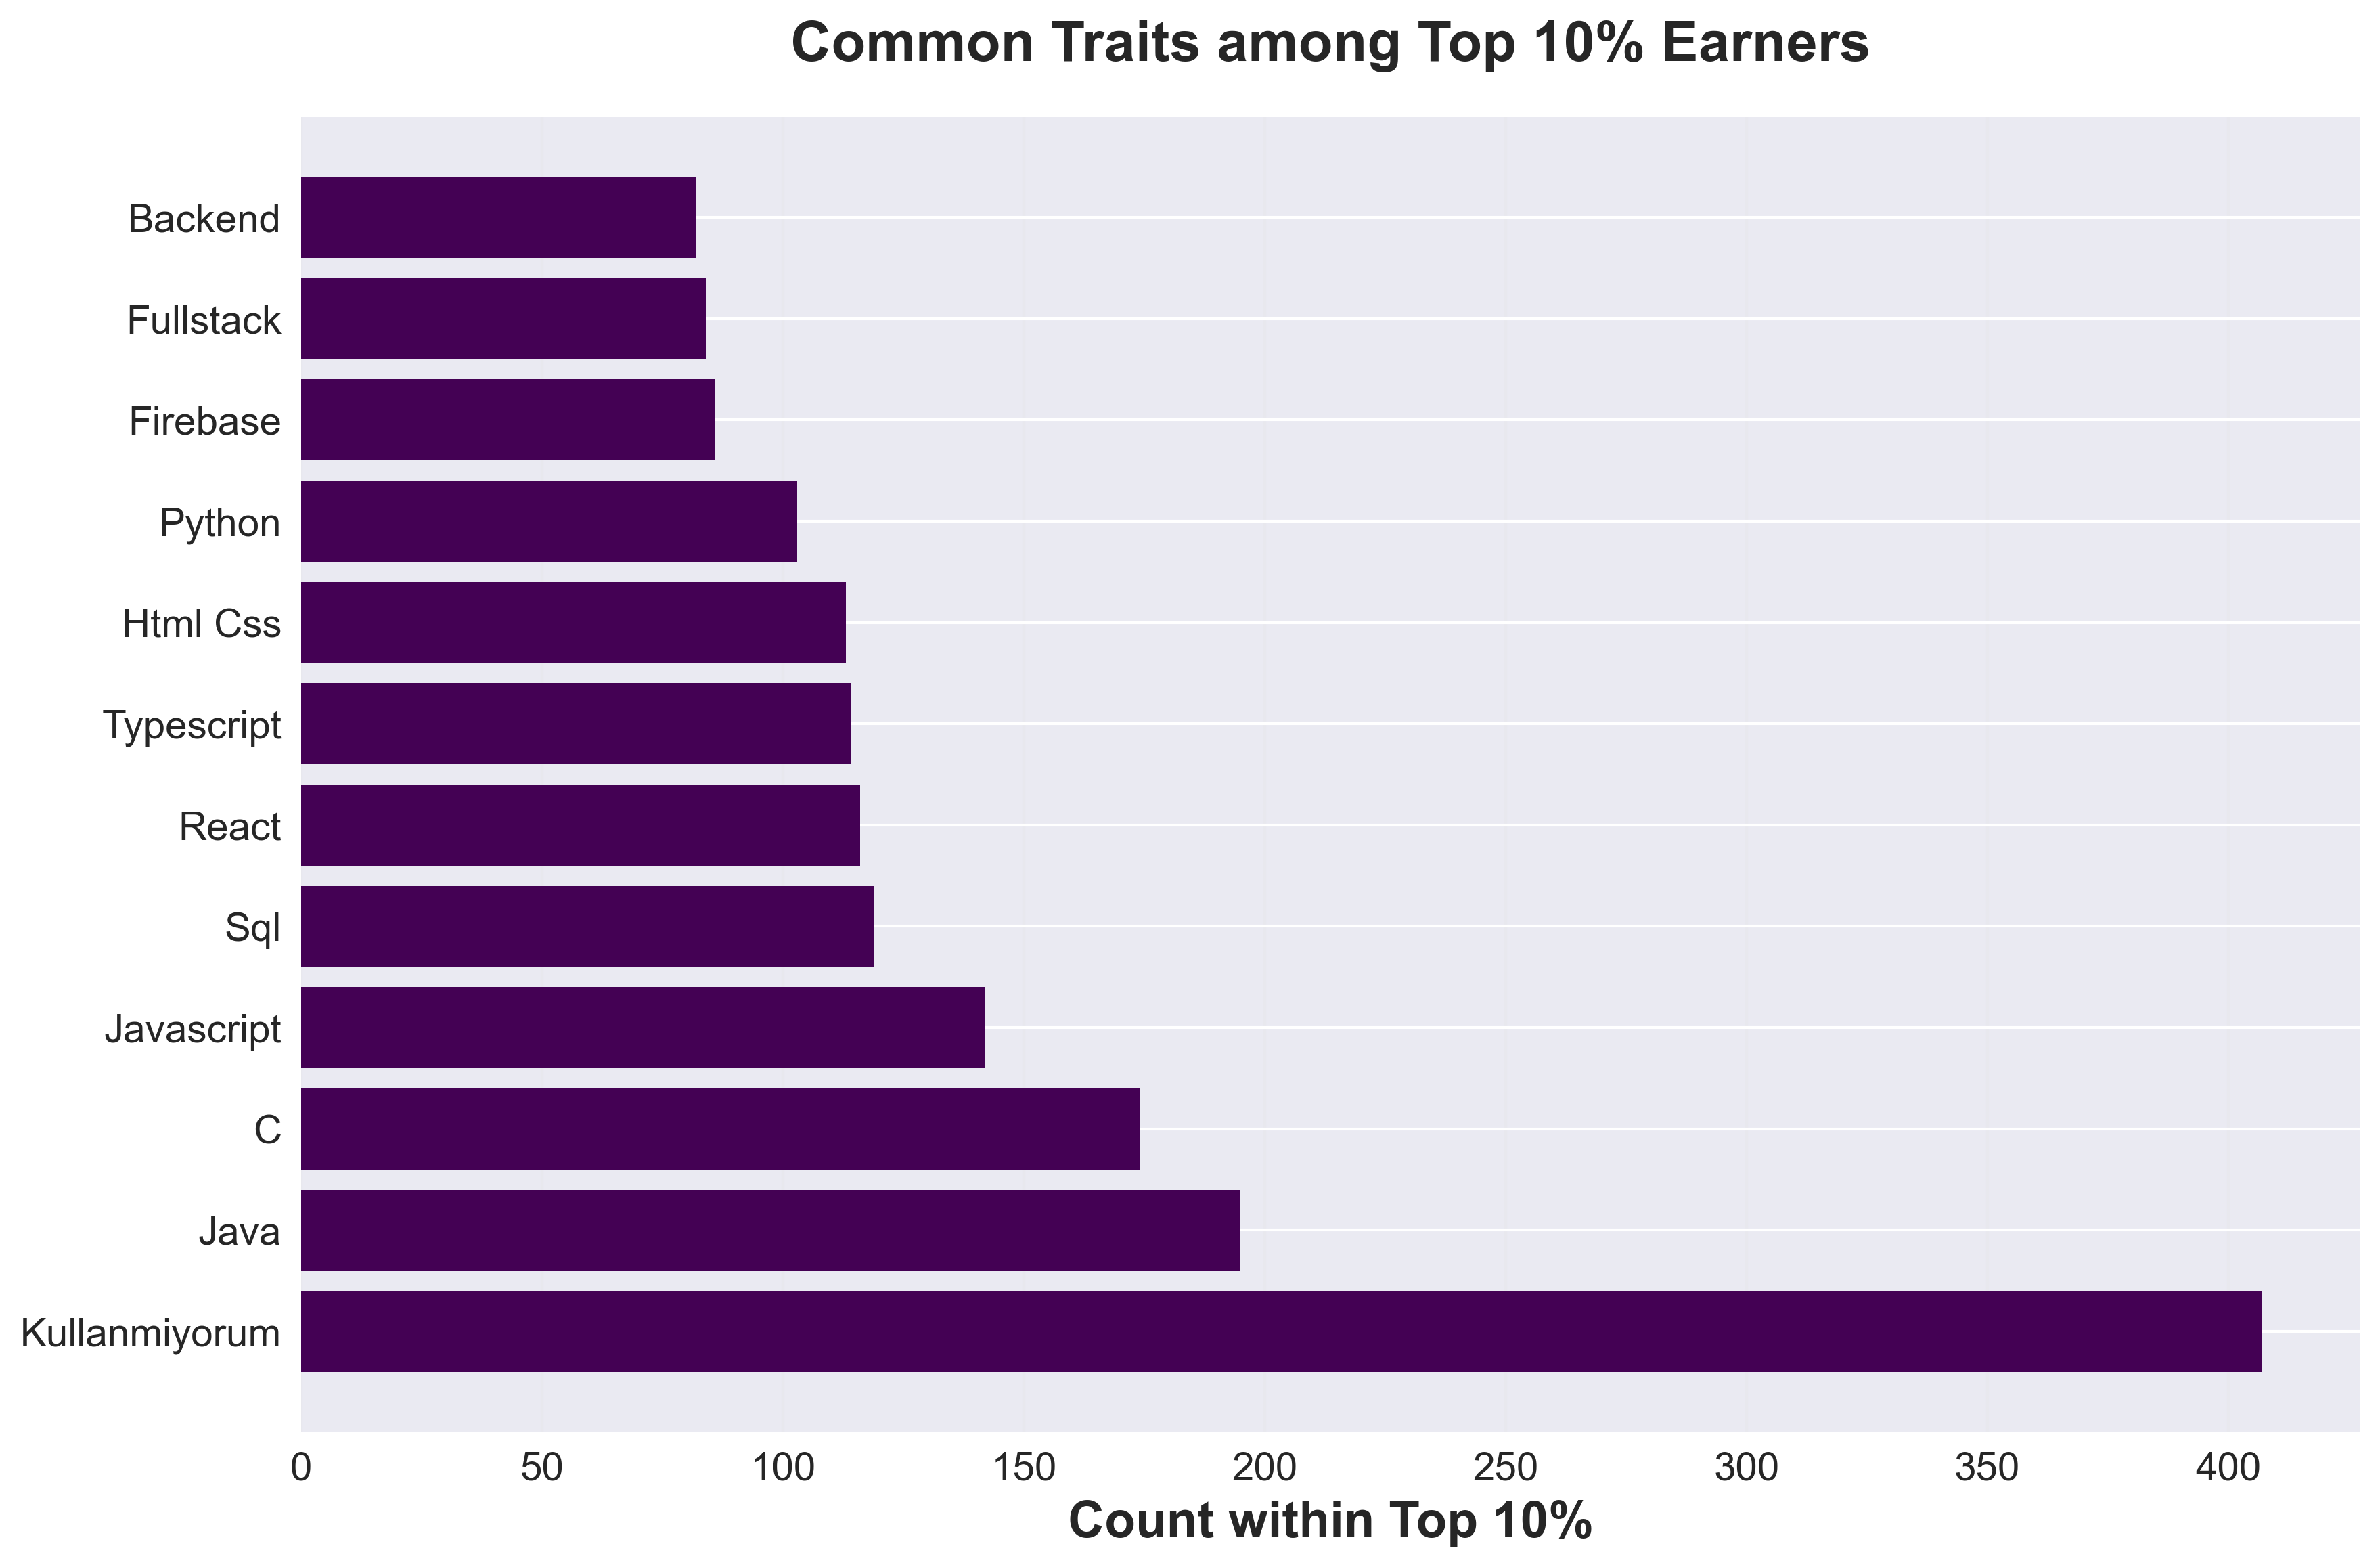
\includegraphics[width=0.85\linewidth]{figures/28_top_earners_traits.png}
  \caption{Common traits among top 10\% earners.}
  \label{fig:top-earners}
\end{figure}
